\documentclass[14pt]{article}
\usepackage[margin=1in]{geometry}
\usepackage{amsmath}
\usepackage{amssymb}
\usepackage{fancyhdr}
\usepackage{graphicx}
\usepackage{xcolor}
\usepackage{tikz}
\usepackage{tikz-3dplot}
\usepackage{chngcntr}
\usepackage{graphicx}
\usepackage{hyperref}
\usepackage{float}
\usetikzlibrary{decorations.pathreplacing}
\usepackage{multicol}
\usepackage{wrapfig}
\tdplotsetmaincoords{70}{110}
\renewcommand{\familydefault}{\sfdefault}
\counterwithin*{equation}{section}
\counterwithin*{equation}{subsection}
\parindent 0ex
\everymath{\displaystyle{}}
\title{Math 277\\Multivariable Calculus for Engineers and Scientists}
\author{Andy Smit}
\date{Winter 2019}

\begin{document}
    \maketitle
    \section{Vector Functions in Two and Three Space}
    subsection{Vector Function: }
    A vector function $\vec{r}$ is a rule that assigns to each real number $t$, one and only one vector 
    $$\begin{pmatrix}x(t)\\  y(t)\\ z(t)\end{pmatrix}$$
    or using the unit vectors $\hat{i}=\left(\begin{smallmatrix}1\\0\\0\end{smallmatrix}\right)$, $\hat{j}=\left(\begin{smallmatrix}0\\1\\0\end{smallmatrix}\right)$ and $\hat{k}=\left(\begin{smallmatrix}0\\0\\1\end{smallmatrix}\right)$,  
    $$x(t)\hat{i}+y(t)\hat{j}+z(t)\hat{k}$$
    and is written 
    \[
        \begin{split}
            \vec{r}(t) &= \begin{pmatrix}x(t)\\y(t)\\z(t)\end{pmatrix}\\ 
            \text{or\ } &= x(t)\hat{i}+y(t)\hat{j}+z(t)\hat{k}
        \end{split}
    \]
    \subsubsection{Geometric Interpretation of a Vector Function:}
    Given a vector function $$\vec{r}(t) = \begin{pmatrix}x(t)\\y(t)\\z(t)\end{pmatrix}$$
    assuming that the functions $x(t)$, $y(t)$, and $z(t)$ are continuous for some interval $I$. The vector function $\vec{r}(t)$, $t\in I$ may be thought of as the position of a moving particle at time $t$ in three-space. As time $t$ varies, the terminal point of the position vector traces a space curve $C$.\\ 
    The space curve $C$ is said to be given parametrically by the vector function $\vec{r}(t)=\left(\begin{smallmatrix}x(t)\\y(t)\\z(t)\end{smallmatrix}\right)$ or is given by the three equations
    $$ \left\{
    \begin{array}{lr}
        x(t)\\
        y(t)\\
        z(t)
    \end{array}
    \right.\ t\in I$$
    \subsubsection{Endpoints and Orientation of a space or Plane Curve:}
    Let $C$ be the space curve given parametrically by the vector function $\vec{r}(t)$, where $t$ is in the closed interval $[a,b]$. The initial and terminal points of the curve $C$ are defined respectively by $\vec{r}(a)$, and $\vec{r}(b)$. Note that if the endpoints coincide the curve $C$ is closed. The orientation of curve $C$ is the direction from the initial point $P$ toward the terminal point $Q$ and is usually denoted with one or two arrow heads.\\\\
    %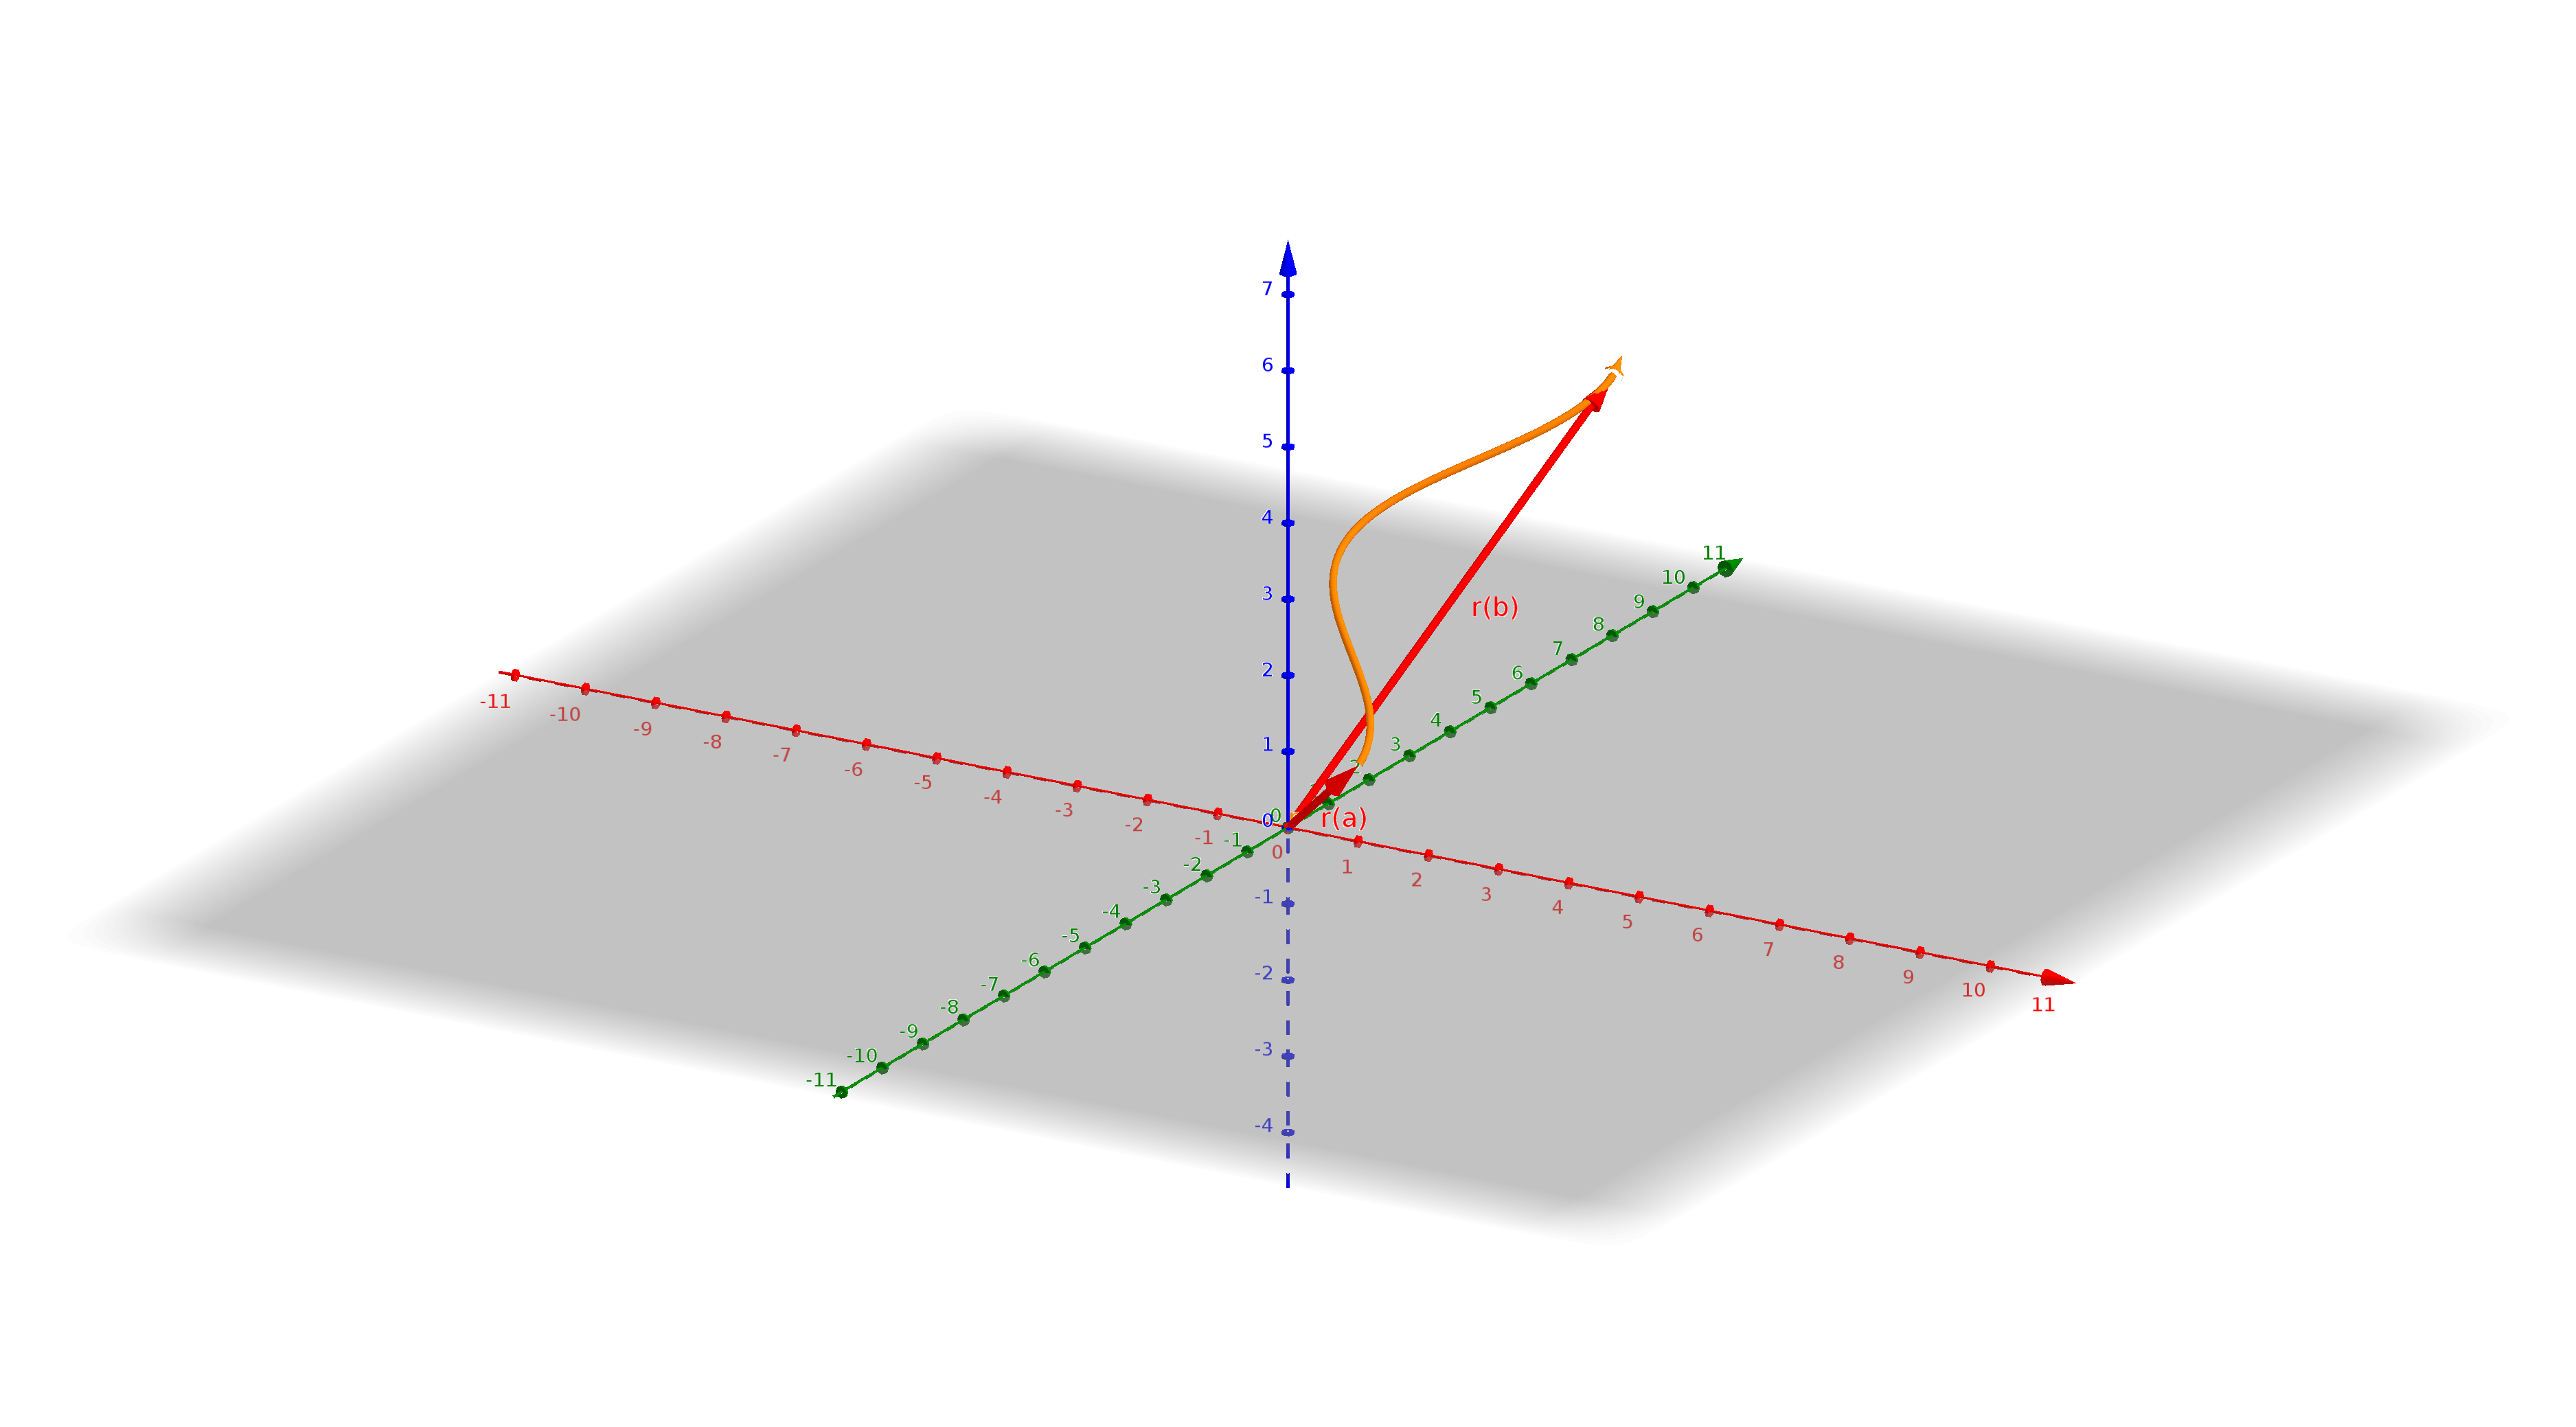
\includegraphics[width=0.5\textwidth]{VectorFunc.png}\\\\
    \subsubsection{Derivative Rules for Vector Functions:}
    let $\vec u(t)$ and $\vec v (t)$ be vector functions with differentiable components and $f(t)$ be a scalar function.\\
    \begin{enumerate}
        \item The sum and difference rule: $\frac{d}{dt}\bigg\{\vec u(t)\pm \vec v(t)\bigg\}=\vec u\ '(t)\pm\vec v\ '(t)$
        \item The scalar Multiple Rule: $\frac{d}{dt}\bigg\{f(t)\vec u(t)\bigg\}=f'(t)\vec u(t)+f(t)\vec u\ '(t)$
        \item The dot Product Rule: $\frac{d}{dt}\bigg\{\vec u(t)\cdot \vec v(t)\bigg\}=\vec u\ '(t)\cdot \vec v(t)+\vec u(t)\cdot \vec v\ '(t)$
        \item The Cross Product Rule: $\frac{d}{dt}\bigg\{\vec u(t)\times \vec v(t)\bigg\}=\vec u\ '(t)\times \vec v(t)+\vec u(t)\times \vec v\ '(t)$
        \item The Chain Rule: $\frac{d}{dt}\bigg\{\vec u(f(t))\bigg\}=\vec u\ '(f(t))f'(t)$
    \end{enumerate}
    \subsection{Motion of a particle in Two and Three-Space}
    \textbf{Position: $\vec r(t)$}\\
    By definition the position of a moving particle at time $t$ is $\vec r(t)$.\\\\
    \textbf{Velocity: $\vec v(t)$}\\
    By definition the average velocity is given by $\vec v_{ave}=\frac{\Delta\vec r(t)}{\Delta t}$. Let $P$ and $Q$ be the position of a particle at time $t$ and $t+\Delta t$ where $\Delta t$ is small. The the velocity of a particle between $P$ and $Q$ is defined, 
    $$\vec v_{P\rightarrow Q}=\frac{Q-P}{t+\Delta t-t}=\frac{\vec r(t+\Delta t)-\vec r(t)}{\Delta t}$$
    If the limit is taken as $\Delta t\rightarrow 0$ then,
    $$\vec v(t)=\lim\limits_{\Delta t\rightarrow 0}\frac{\vec r(t+\Delta t)-\vec r(t)}{\Delta t}=\frac{d\vec r}{dt}=\vec r\ '(t)$$
    It follows that the tangent line to the curve $C$ at $P$ is in the direction of the velocity vector at $P$.
    $$\vec v(t)=\frac{d\vec r}{dt}= \frac{dx}{dt}\hat i+ \frac{dy}{dt}\hat j +\frac{dz}{dt}\hat k$$
    \textbf{Acceleration: $\vec a(t)$}\\
    By definition the acceleration is the derivative of velocity with respect to time,
    $$\vec a (t)=\frac{d\vec v}{dt}=\frac{d^2\vec r}{dt^2}$$
    \textbf{Speed: $v(t)$}\\
    By definition the speed is the magnitude or norm of the velocity,
    $$v(t)=||\vec v (t)||$$
    \textbf{Distance Traveled: $L$}\\
    The distance traveled or arc length of a curve on the interval $[a,b]$ is denoted and defined
    $$L=\int\limits_a^bv\, dt=\int\limits_a^b\sqrt{\frac{dx}{dt}^2+\frac{dy}{dt}^2+\frac{dz}{dt}^2}\, dt$$
    \subsection{Special Parametric Curves:}
    \textbf{The Straight Line Segment}
    \begin{multicols}{2}
        Recall the parametric Vector equation of a Straight Line 
        $$\vec r (t)=\vec{r_0}=t\vec v,\ t\in\mathbb{R}$$
        Here $\vec{r_0}$ is equivilant to the point $P=(x_1,y_1)$ and $\vec v=\begin{pmatrix} x_2-x_1\\y_2-y_1\end{pmatrix}$.
        $$\therefore \vec r(t)=\begin{pmatrix}x_1\\ y_1\end{pmatrix}+t\begin{pmatrix}x_2-x_1\\y_2-y_1\end{pmatrix},\ t\in\mathbb{R}$$
        If follows that the parametric vector equation of the straight line segment with initial point $P=(x_1,y_1)$ and terminal point $Q=(x_2, y_2)$ is given by
        $$\vec r(t)=\begin{pmatrix}x_1\\ y_1\end{pmatrix}+t\begin{pmatrix}x_2-x_1\\y_2-y_1\end{pmatrix},\ t\in[0,1]$$
        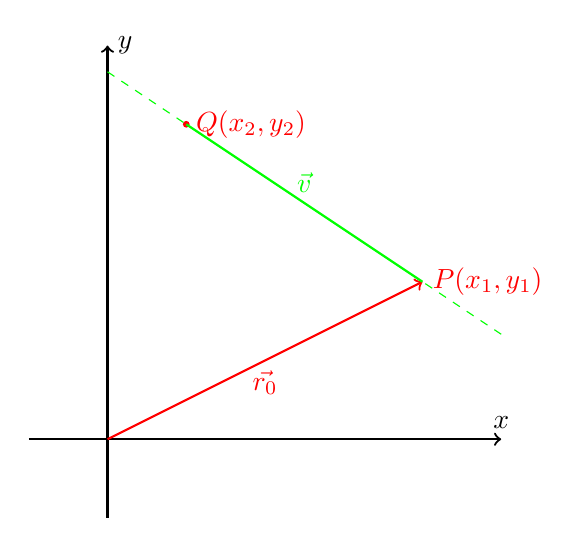
\begin{tikzpicture}[domain=0:5]
            \draw[thick, ->](-1,0)-- (5,0) node[above]{$x$};
            \draw[thick, ->](0,-1)-- (0,5) node[right]{$y$};
            \draw[red,thick, ->] (0,0)--(4,2) node[midway, below]{$\vec{r_0}$} node[right]{$P(x_1,y_1)$};
            \filldraw[red] (1,4) circle(1pt) node[right]{$Q(x_2,y_2)$};
            \draw[dashed, green] plot(\x, {-2/3*\x+4+2/3});
            \draw[thick, green] (4,2)--(1,4) node[midway, above]{$\vec v$};
        \end{tikzpicture}\\
    \end{multicols}   
    \textbf{The Ellipse}
    \begin{multicols}{2}
        The parametric vector equation of an ellipse with center at $(h,k)$ and with semi-axis length of $a$, $b$ is given by
        $$\vec r(t)=(h+a\cos(t))\hat i+(k+b\sin(t))\hat j,\ t\in[0,2\pi]$$
        or parametrically as 
        $$\frac{(x-h)^2}{a^2}+\frac{(y-k)^2}{b^2}=1$$
        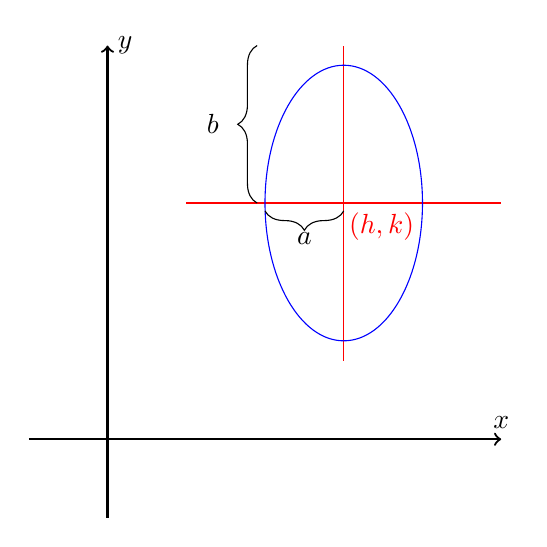
\begin{tikzpicture}[domain=0:5]
            \draw[thick, ->](-1,0)-- (5,0) node[above]{$x$};
            \draw[thick, ->](0,-1)-- (0,5) node[right]{$y$};
            \draw[thin, red](1,3)--(5,3) node[pos=0.62, below]{$(h,k)$};
            \draw[thin, red](3,1)--(3,5);
            \draw[blue] (3,3) ellipse(1 and 1.75);
            \draw [decorate,decoration={brace,amplitude=7pt}] (1.9,3)--(1.9,5) node[midway, xshift=-16pt]{$b$};
            \draw [decorate, decoration={brace, amplitude=7pt,mirror}] (2, 2.9)--(3,2.9) node[midway, yshift=-10pt]{$a$};
        \end{tikzpicture}\\
    \end{multicols}
    \textbf{The Circle}
    \begin{multicols}{2}
        The parametric vector equation of a circle centered at $(h,k)$ with radius $a$ is given by
        $$\vec r(t)=(h+a\cos(t))\hat i+(k+b\sin(t))\hat j$$
        or parametrically as
        $$(x-h)^2+(y-k)^2=a^2$$
        \begin{tikzpicture}[domain=0:5]
            \draw[thick, ->](-1,0)-- (5,0) node[above]{$x$};
            \draw[thick, ->](0,-1)-- (0,5) node[right]{$y$};
            \draw[blue] (3,3) circle(1.5);
            \draw[thin, red](1,3)--(5,3) node[pos=0.62, below]{$(h,k)$};
            \draw[thin, red](3,1)--(3,5);
        \end{tikzpicture}\\
    \end{multicols}
    \textbf{The Hyperbola}
    \begin{multicols}{2}
        The parametric vector equation of the right hand branch of a hyperbola with center at $(h,k)$, semi transverse axis of length $a$ and semi conjugate axis of length $b$ is given by
        $$\vec r(t)=(h+a\cosh(t))\hat i+(k+b\sinh(t))\hat j, t\in\mathbb{R}$$ 
        or parametrically as
        $$\frac{(x-h)^2}{a^2}-\frac{(y-k)^2}{b^2}=1$$
        \begin{tikzpicture}[domain=0:5]
            \draw[thick, ->](-1,0)-- (5,0) node[above]{$x$};
            \draw[thick, ->](0,-1)-- (0,5) node[right]{$y$};
            \draw[blue, domain=-1.3:1.3] plot({3+cosh(\x)}, {3+sinh(\x)});
            \draw[blue, domain=-1.3:1.3] plot({3-cosh(\x)}, {3+sinh(\x)});
            \draw[thin, red](1,3)--(5,3) node[pos=0.62, below]{$(h,k)$};
            \draw[thin, red](3,1)--(3,5);
        \end{tikzpicture}\\
    \end{multicols}
    \textbf{The Parabola}
    \begin{multicols}{2}
        There is no standard parametric vector equation for a parabola. There instead are infinitely many parametric vector equations for a parabola. To find a parametric vector equation for a parabola simply assign any value for $x$, or $y$ asa long as the values of $x$ and $y$ are not restricted. The cartesian equations of a parabola are
        \begin{align*}
            &y=ax^2+bx+c,& a\neq 0\\
            \mathrm{or}\ & x=ay^2+by+c,& a\neq 0
        \end{align*}
        \begin{tikzpicture}[domain=-1:3]
            \draw[thick, ->](-1,0)-- (5,0) node[above]{$x$};
            \draw[thick, ->](0,-1)-- (0,5) node[right]{$y$};
            \draw[blue] plot(\x, {(\x)^2-(\x)-1});
        \end{tikzpicture}\\
    \end{multicols}
    \subsection{Special Parametric Curves in Space:}
    \textbf{The Straight Line Segment:}\\
    The parametric Vector equation of the straight line segment given by the points $P(x_1, y_1, z_1)$ and $Q(x_2, y_2, z_2)$ is given by 
    $$\vec r= \vec{r_0}+t\vec v,\ t\in[0,1]$$\
    Where $\vec{r_0}=P$ and $\vec v=\vec{PQ}$ or parametrically as
    $$\vec r(t)=\left\{\begin{array}{lr}
        x=x_1+(x_2-x_1)t\\
        y=y_1+(y_2-y_1)t\\
        z=z_1+(z_2-z_1)t
    \end{array}\right.$$
    \textbf{The Helix:}\\
    A Helix is a wire wrapped around the surface of a cylinder. If the cylinder is a right circular cylinder with radius $a$ and height $b$, then the parametric vector equation of the helix is given by
    $$\vec r(t)=\begin{pmatrix}
        a\cos(t)\\
        a\sin(t)\\
        bt
    \end{pmatrix},\ t\in[0,2\pi]$$
    \subsection{General Curves in Space:}
    A space curve C is the intersection of 2 surfaces, say $S_1$ and $S_2$. For instance
    \begin{enumerate}
        \item The intersection of 2 planes is a straight line
        \item The intersection of a cone and a plane generates a conic section (circle, an ellipse, a parabola, a hyperbola, or a pair of lines.)
    \end{enumerate}
    Let $C$ be the curve of intersection of $S_1$ and $S_2$ where
    \begin{equation}\label{S1}
        S_1:f(x,y,z)=0
    \end{equation}
    \begin{equation}\label{S2}
        S_2:g(x,y,z)=0
    \end{equation}
    To find the parametric vector equation of the space curve $C$, attempt to use equations \eqref{S1} and \eqref{S2} to obtain a third equation consisting of only two of the three variables. When this equation is viewed in $\mathbb{R}^2$ (the xy-plane, xz-plane or yz-plane), it can easily be parametrized.
    \subsection{The $\vec T$, $\vec N$, and $\vec B$ Frame}
    First Recall the definition of a unit vector. If If $\vec v$ is a vector in $\mathbb{R}^n$, then $\vec v$ is a unit vector if and only if the length of $v$ is 1. Let $C$ be a plane or space curve given by the vector function $\vec r(t),\ t\in I$ and let $P$ be a point on curve $C$.
    \subsubsection{The Unit Tangent Vector: $\vec T(t)$}
    The unit tangent vector to curve $C$ at $P$ is denoted and defined by
    $$\vec T(t)=\frac{\vec v(t)}{||\vec v (t)||}$$
    $\vec T(t)$ is a unit vector in the direction of the velocity and hence is tangent to the curve $C$ at $P$ and points in the orientation of $C$.
    \subsubsection{The Principle Unit Normal: $\vec N(t)$}
    The principle unit vector to the curve $C$ at $P$ is denoted and defined by
    $$\vec N(t)=\frac{\vec T(t)}{||\vec T(t)||}$$
    \subsubsection{The Curvature: $\kappa$}
    Given $\vec r(t)$ the rate of turn is given by $$\kappa=\left|\left|\frac{d\vec T}{ds}\right|\right|$$ where $s$ denotes the arc length. This is the scalar quantity representing the change in $\vec T$ with respect to distance  travelled. This is called the curvature $\kappa$. The curvature $\kappa$ can also be defined as
    $$\kappa=\frac{\vec{v}\times\vec{a}}{v^3}$$
    \subsubsection{The Radius of Curvature $\rho$}
    At a point $P$ on a curve $C$ we define the radius of curvature by
    $$\rho=\frac{1}{\kappa}$$
    The circle of radius $\rho$ tangent to curve $C$ at $P$ on the concave side is called the circle of curvature.
    \subsubsection{The Unit Binormal Vector: $\vec B$}
    The cross product of $\vec T$ and $\vec N$ is a vector orthogonal to both $\vec T$ and $\vec N$. This vector is denoted $\vec B(t)$ and is defined
    $$\vec B(t)=\vec T(t)\times \vec N(t)$$
    The vector $\vec B$ is called the Unit Binormal Vector. Geometrically the $\vec T$, $\vec N$, and $\vec B$ vector determine the spacial properties of direction of travel, turn, and twist respectively of the curve $C$.
    \subsubsection{The Torsion: $\tau$}
    The torsion $\tau$ of a space curve $C$ is denoted and defined by 
    $$\tau=-\frac{d\vec B}{ds}\cdot\vec N$$
    Geometrically the torsion provides a measure of the degree of twisting of a space curve. Given a curve $C=\vec r(t)$ the torsion can also be defined
    $$\tau=\frac{(\vec v\times \vec a)\cdot\vec a\,'}{||\vec v\times\vec a||^2}$$
    \subsection{Tangential and Normal Components of Acceleration}
    Let $a_T=\frac{dv}{dt}$ and $a_N=\kappa v^2$
    \begin{align*}
        \therefore \vec a(t)&=a_T \vec T+ a_N \vec N\\
        &=\frac{dv}{dt}\vec T+\kappa v^2\vec N
    \end{align*}
    The scalars $a_T$ and $a_N$ are respectively called the tangent component and normal component of acceleration.
    \subsubsection{Alternative formula for the Tangent and Normal components of Acceleration}
    The normal component of acceleration can be given by
    $$a_N=\frac{||\vec v\times \vec a||}{v}$$
    The tangential component of acceleration can be given by
    $$a_T=\vec T\cdot\vec a =\frac{\vec v\cdot \vec a}{v}$$
    \subsection{Summary and alternative Formula of $\vec T$, $\vec N$, $\vec B$, $\kappa$, $\rho$, $\tau$, $a_T$, and $a_N$}
    \begin{align}
        \vec T=\frac{\vec v}{v}\\
        \vec B=\frac{\vec v\times\vec a}{||\vec v\times \vec a||}\\
        \vec N=\vec B\times \vec T\\
        \kappa=\frac{||\vec v\times \vec a||}{v^3}\\
        \rho=\frac{1}{\kappa}\\
        \tau=\frac{(\vec v\times \vec a)\cdot\vec a\, '}{||\vec v\times \vec a||^2}\\
        a_N=\frac{||\vec v\times \vec a||}{v}\\
        a_T=\vec T\cdot\vec a =\frac{\vec v\cdot \vec a}{v}\\
        \vec T=\vec N\times\vec B\\
        \vec B=\vec B\times N
    \end{align}
    \subsection{Applications of Vector Functions}
    \subsubsection{The Rocket Equation}
    A rocket moves forward by the backward expulsion of a mass of gas formed by burning its onboard fuel.
    \begin{enumerate}
        \item $M$: The total initial mass of the rocket including its fuel.
        \item $m=m(t)$: total mass of the rocket at time $t$. Hence $m+\Delta m$ is the total mass of the rocket at time $t+\Delta t$. It follows that $\Delta m<0$ and $-\Delta m>0$. Therefore the amount of fuel burnet over a time interval $\Delta t$ is $-\Delta m$.
        \item $\vec v=\vec v(t)$: The velocity of the rocket at time $t$ relative to the earth. Hence $\vec v+\Delta\vec v$ is the velocity at time $t+\Delta t$
        \item $-\vec{v_e}$: The velocity of the ejected gas (assume constant). It follows that $\vec v+\vec{v_e}$ is the velocity of the ejected gas relative to the earth.
        \item $\alpha$: The rate at which the fuel mixture is burned in the rocket (assume constant).\\
        $$\therefore-\alpha=\frac{dm}{dt}\Rightarrow m=\int\alpha\, dt=-\alpha t+M$$ or
        \begin{equation}\label{mass}
            m(t)=M-\alpha t
        \end{equation}
        \item $\vec F$: The net force acting on the rocket
        \item $\vec p(t)$ The momentum of the rocket. $\vec p(t)=m\vec v$. Hence the change in momentum over time is thus given by
    \end{enumerate}
    \begin{align*}
        \Delta\vec p&=\vec p(t+\Delta t)-\vec p(t)\\
        &=\big[(m+\Delta m)(\vec v+\Delta\vec v)+(-\Delta m)(\vec v+\vec {v_e})\big]-m\vec v\\
        &=\big[m\vec v+m\Delta\vec v+\vec v\Delta m+\Delta m\Delta\vec v-\vec v\Delta m-\vec{v_e}\Delta m\big]-m\vec v\ \text{\footnotemark}\\
        &=m\Delta\vec v-\Delta m\, \vec v_e\\
        \frac{\Delta\vec p}{\Delta t}&=m \frac{\Delta\vec v}{\Delta t}-\vec{v_e}\frac{\Delta m}{\Delta t}\\
        \lim\limits_{\Delta\rightarrow0}\frac{\Delta\vec p}{\Delta t}&=m \lim\limits_{\Delta\rightarrow0}\frac{\Delta\vec v}{\Delta t}-\vec{v_e}\lim\limits_{\Delta\rightarrow0}\frac{\Delta m}{\Delta t}\\
    \end{align*}
    \footnotetext{Note $\Delta m\Delta v$ is very small and is therefore omitted}
    \begin{equation}\label{momentum}
        \frac{d\vec p}{d t}=m \frac{d\vec v}{d t}-\vec{v_e}\frac{d m}{d t}
    \end{equation}
    Apply Newtons second law of motion, the derivative of momentum with respect to time is $\vec F=\frac{d\vec p}{dt}$, to \eqref{momentum} to obtain
    \begin{equation}\label{Force1}
        \vec F=m \frac{d\vec v}{d t}-\vec{v_e}\frac{d m}{d t}\\
    \end{equation}
    Assumptions
    \begin{enumerate}
        \item Assume the rocket moves in a straight line vertically upward. Hence $\vec F=0\rightarrow F=0\hat k$, $\vec v=v\hat k$, $v$ being the speed of the rocket relative to the earth, and $\vec{v_e}=-v_e\hat k$, $v_e$ being the speed of the ejected gas relative to the rocket.
        \item The rocket is initially at rest. Hence $M=m(t)$ when $v=$.
    \end{enumerate}
    Substitute for $v$, $v_e$, and $F$ from the above assumptions into \eqref{Force1}
    \begin{align*}
        0&=m\frac{dv}{dt}-v_e\frac{dm}{dt}\\
        m\, \frac{dv}{dt}&=-v_e\frac{dm}{dt}   
    \end{align*}
    \begin{equation}\label{dv}
        \frac{dv}{dt}=-\frac{v_e} {m}\frac{dm}{dt}
    \end{equation}
    Integrate both sides of \eqref{dv}
    \begin{align*}
        \int\limits_0^t \frac{dv}{dt}\, dt&=\int\limits_0^t -\frac{v_e} {m}\frac{dm}{dt}\, dt\\
        v(t)-v(0)&=-v_e\ln(m(t))+v_e\ln(m(0))
    \end{align*}
    Therefore the velocity of a rocket at time $t$ is given by
    \begin{equation}\label{rocket}
        v(t)=v_e\ln\left(\frac{M}{m(t)}\right)
    \end{equation}
    Subbing in \eqref{mass} into \eqref{rocket} then gives
    $$v(t)=v_e\ln\left(\frac{M}{M-\alpha t}\right)$$
    
    \subsubsection{Banking of a Road Turn:}
    If a road is straight, its design is horizontal. However, when on a sharp turn it becomes angled. This design is referred to as banking of a road turn. Banked road turns have a rated speed limit that must be followed in order to use the road safely. Here we shall only look at frictionless roads. If a curve is banking at an angle $\theta$, with a radius of curvature $\rho$ and a rated speed of $v$, then the quantities are related by
    $$\tan \theta=\frac{v^2}{g\rho}$$ 
    \pagebreak
    \section{Functions of Several Variables}
    \subsection{Quadric Surfaces:}
    A quadratic equation in $x$, $y$, and $z$ is called a quadric surface. Quadric surfaces may be thought of as three dimensional versions of conic sections.
    Let $a$, $b$, and $c$ be positive
    \subsubsection{The Ellipsoid Family:}
    \textbf{The Ellipsoid:}
    \begin{multicols}{2}
        \begin{equation}
            \frac{x^2}{a^2}+\frac{y^2}{b^2}+\frac{z^2}{c^2}=1
        \end{equation}
        The ellipsoid is centered at $(0, 0, 0)$ and has semi axis $a$, $b$, and $c$.\\
        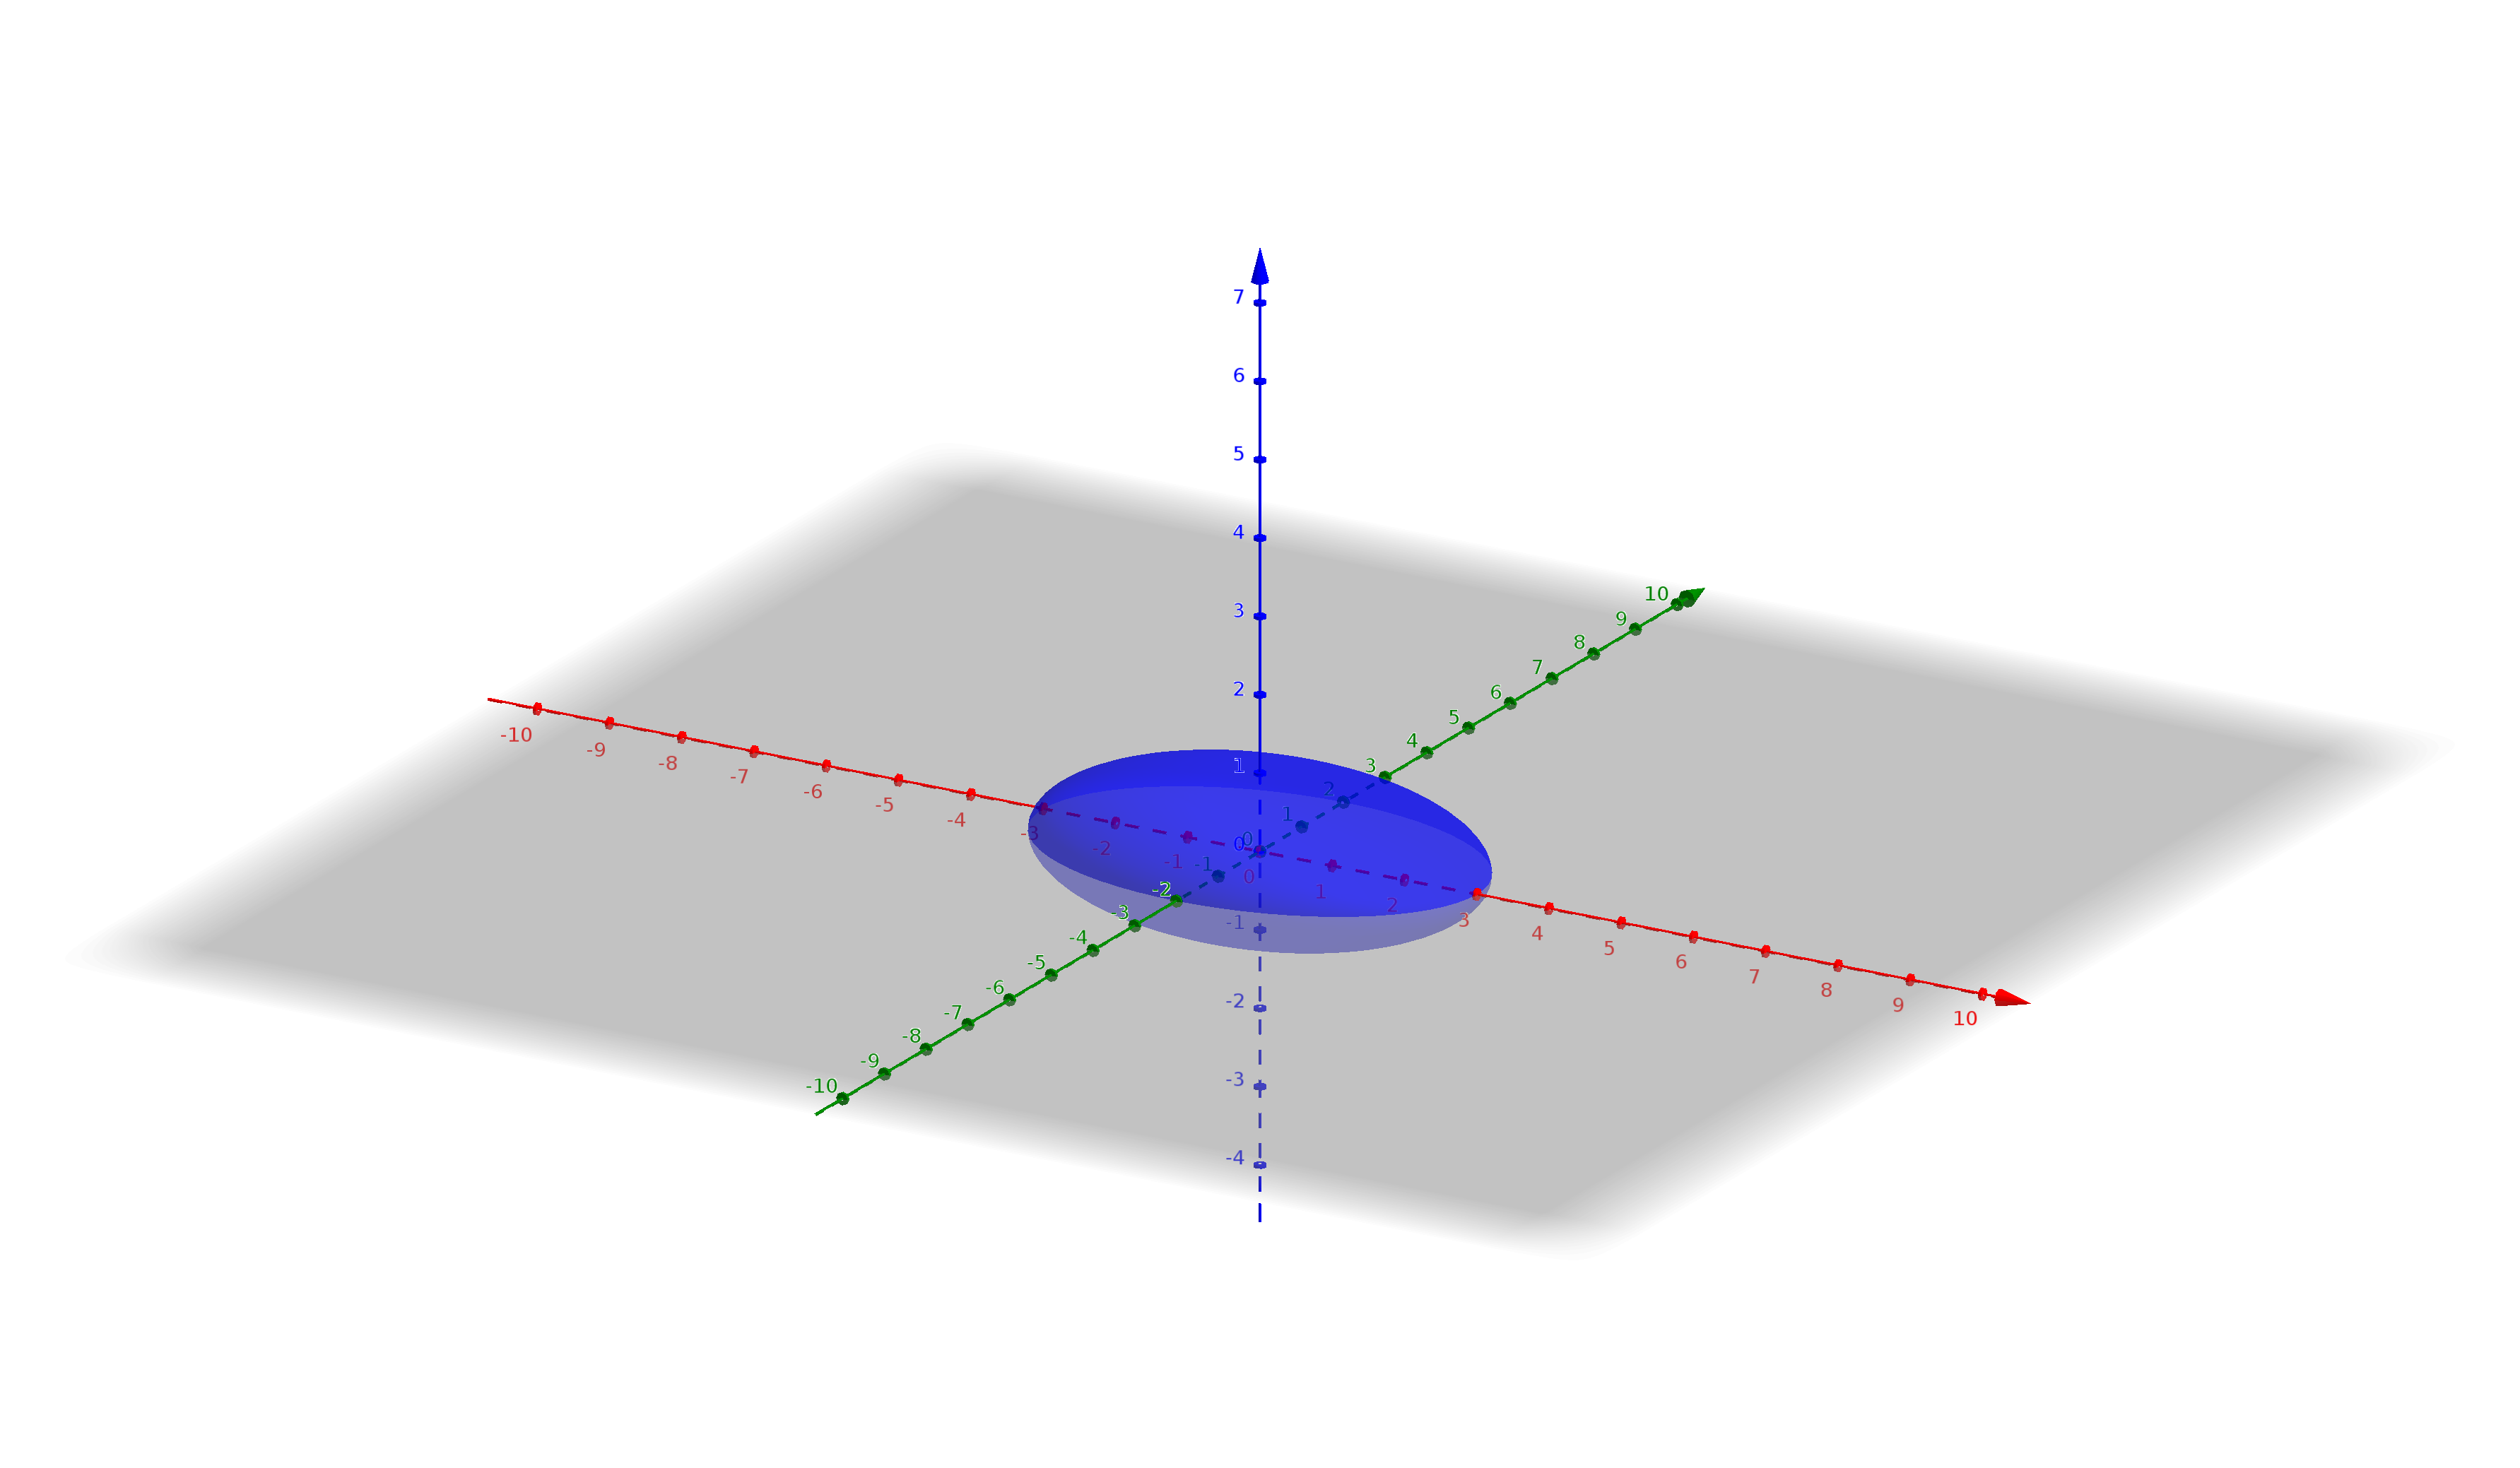
\includegraphics[width=0.5\textwidth]{Ellipsoid.png}
    \end{multicols}
    \textbf{The Sphere:}
    \begin{multicols}{2}
        \begin{equation}
            x^2+y^2+z^2=a^2
        \end{equation}
        The sphere is centered at $(0,0,0)$ and has radius $a$\\
        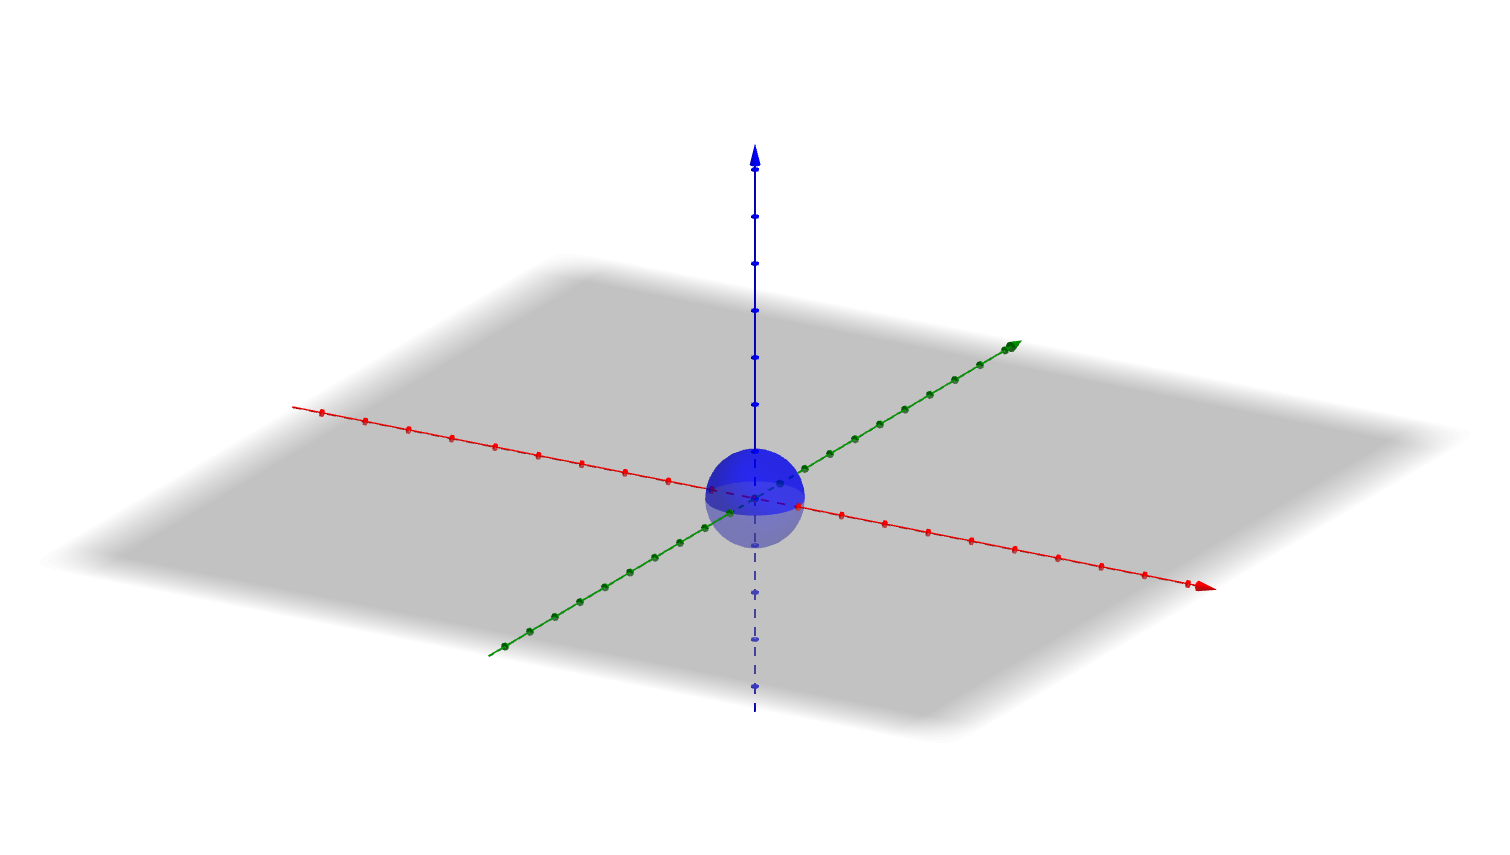
\includegraphics[width=0.5\textwidth]{Sphere.png}    
    \end{multicols}
    \pagebreak
    \subsubsection{The Paraboloid Family:}
    \textbf{The Elliptic Paraboloid:}
    \begin{multicols}{2}
        \begin{equation}z=\pm\left(\frac{x^2}{a^2}+\frac{y^2}{b^2}\right)\end{equation}    
        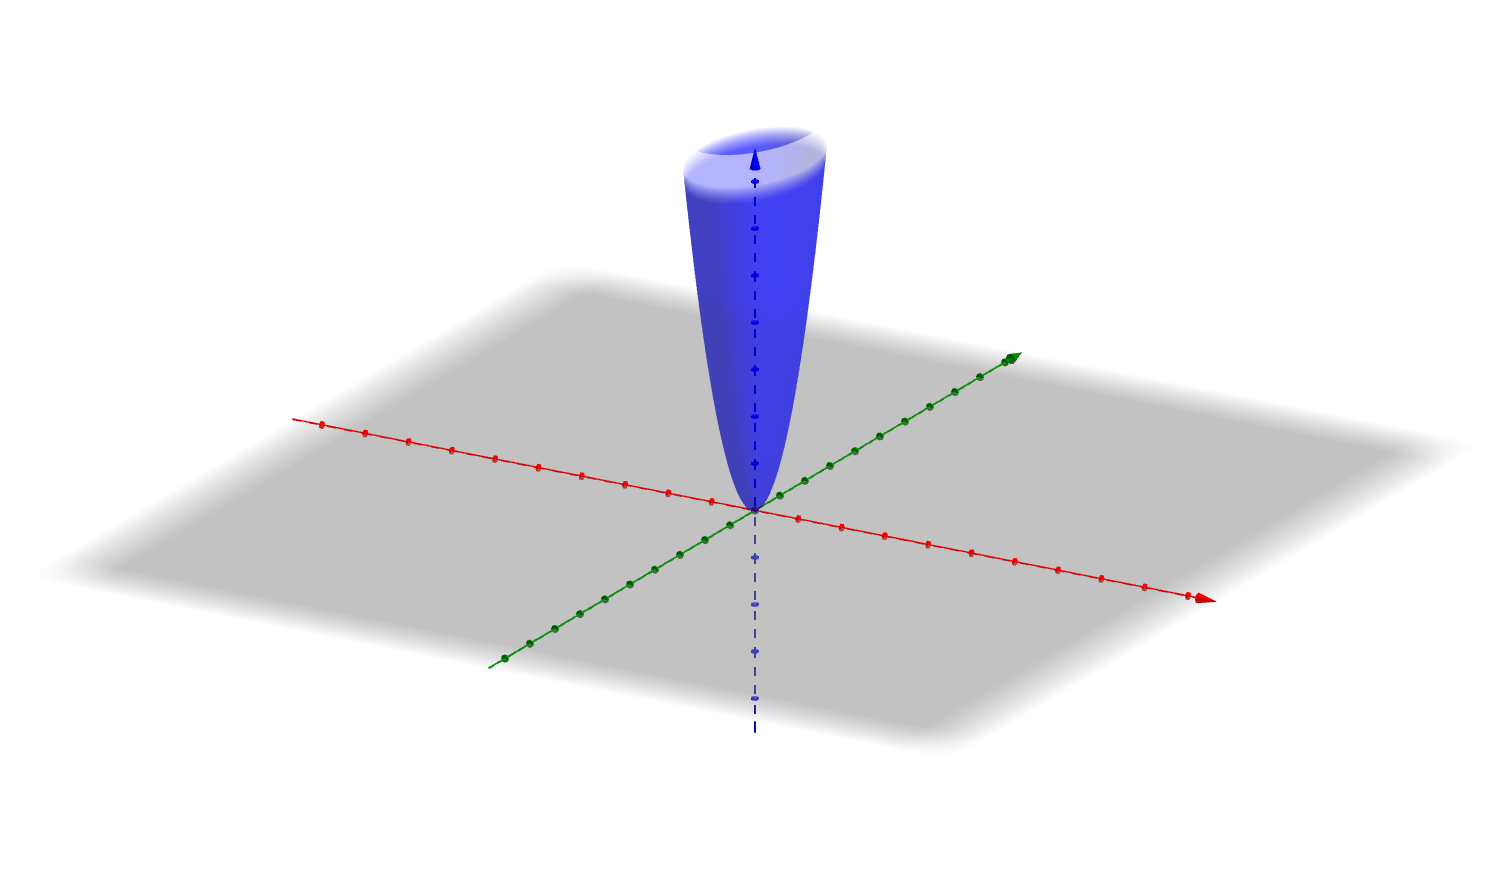
\includegraphics[width=0.5\textwidth]{Elliptical_Paraboloid.png}
    \end{multicols}
    \textbf{The Circular Paraboloid:}
    \begin{multicols}{2}
        \begin{equation}z=\pm\left(\frac{x^2}{a^2}+\frac{y^2}{a^2}\right)\end{equation}
        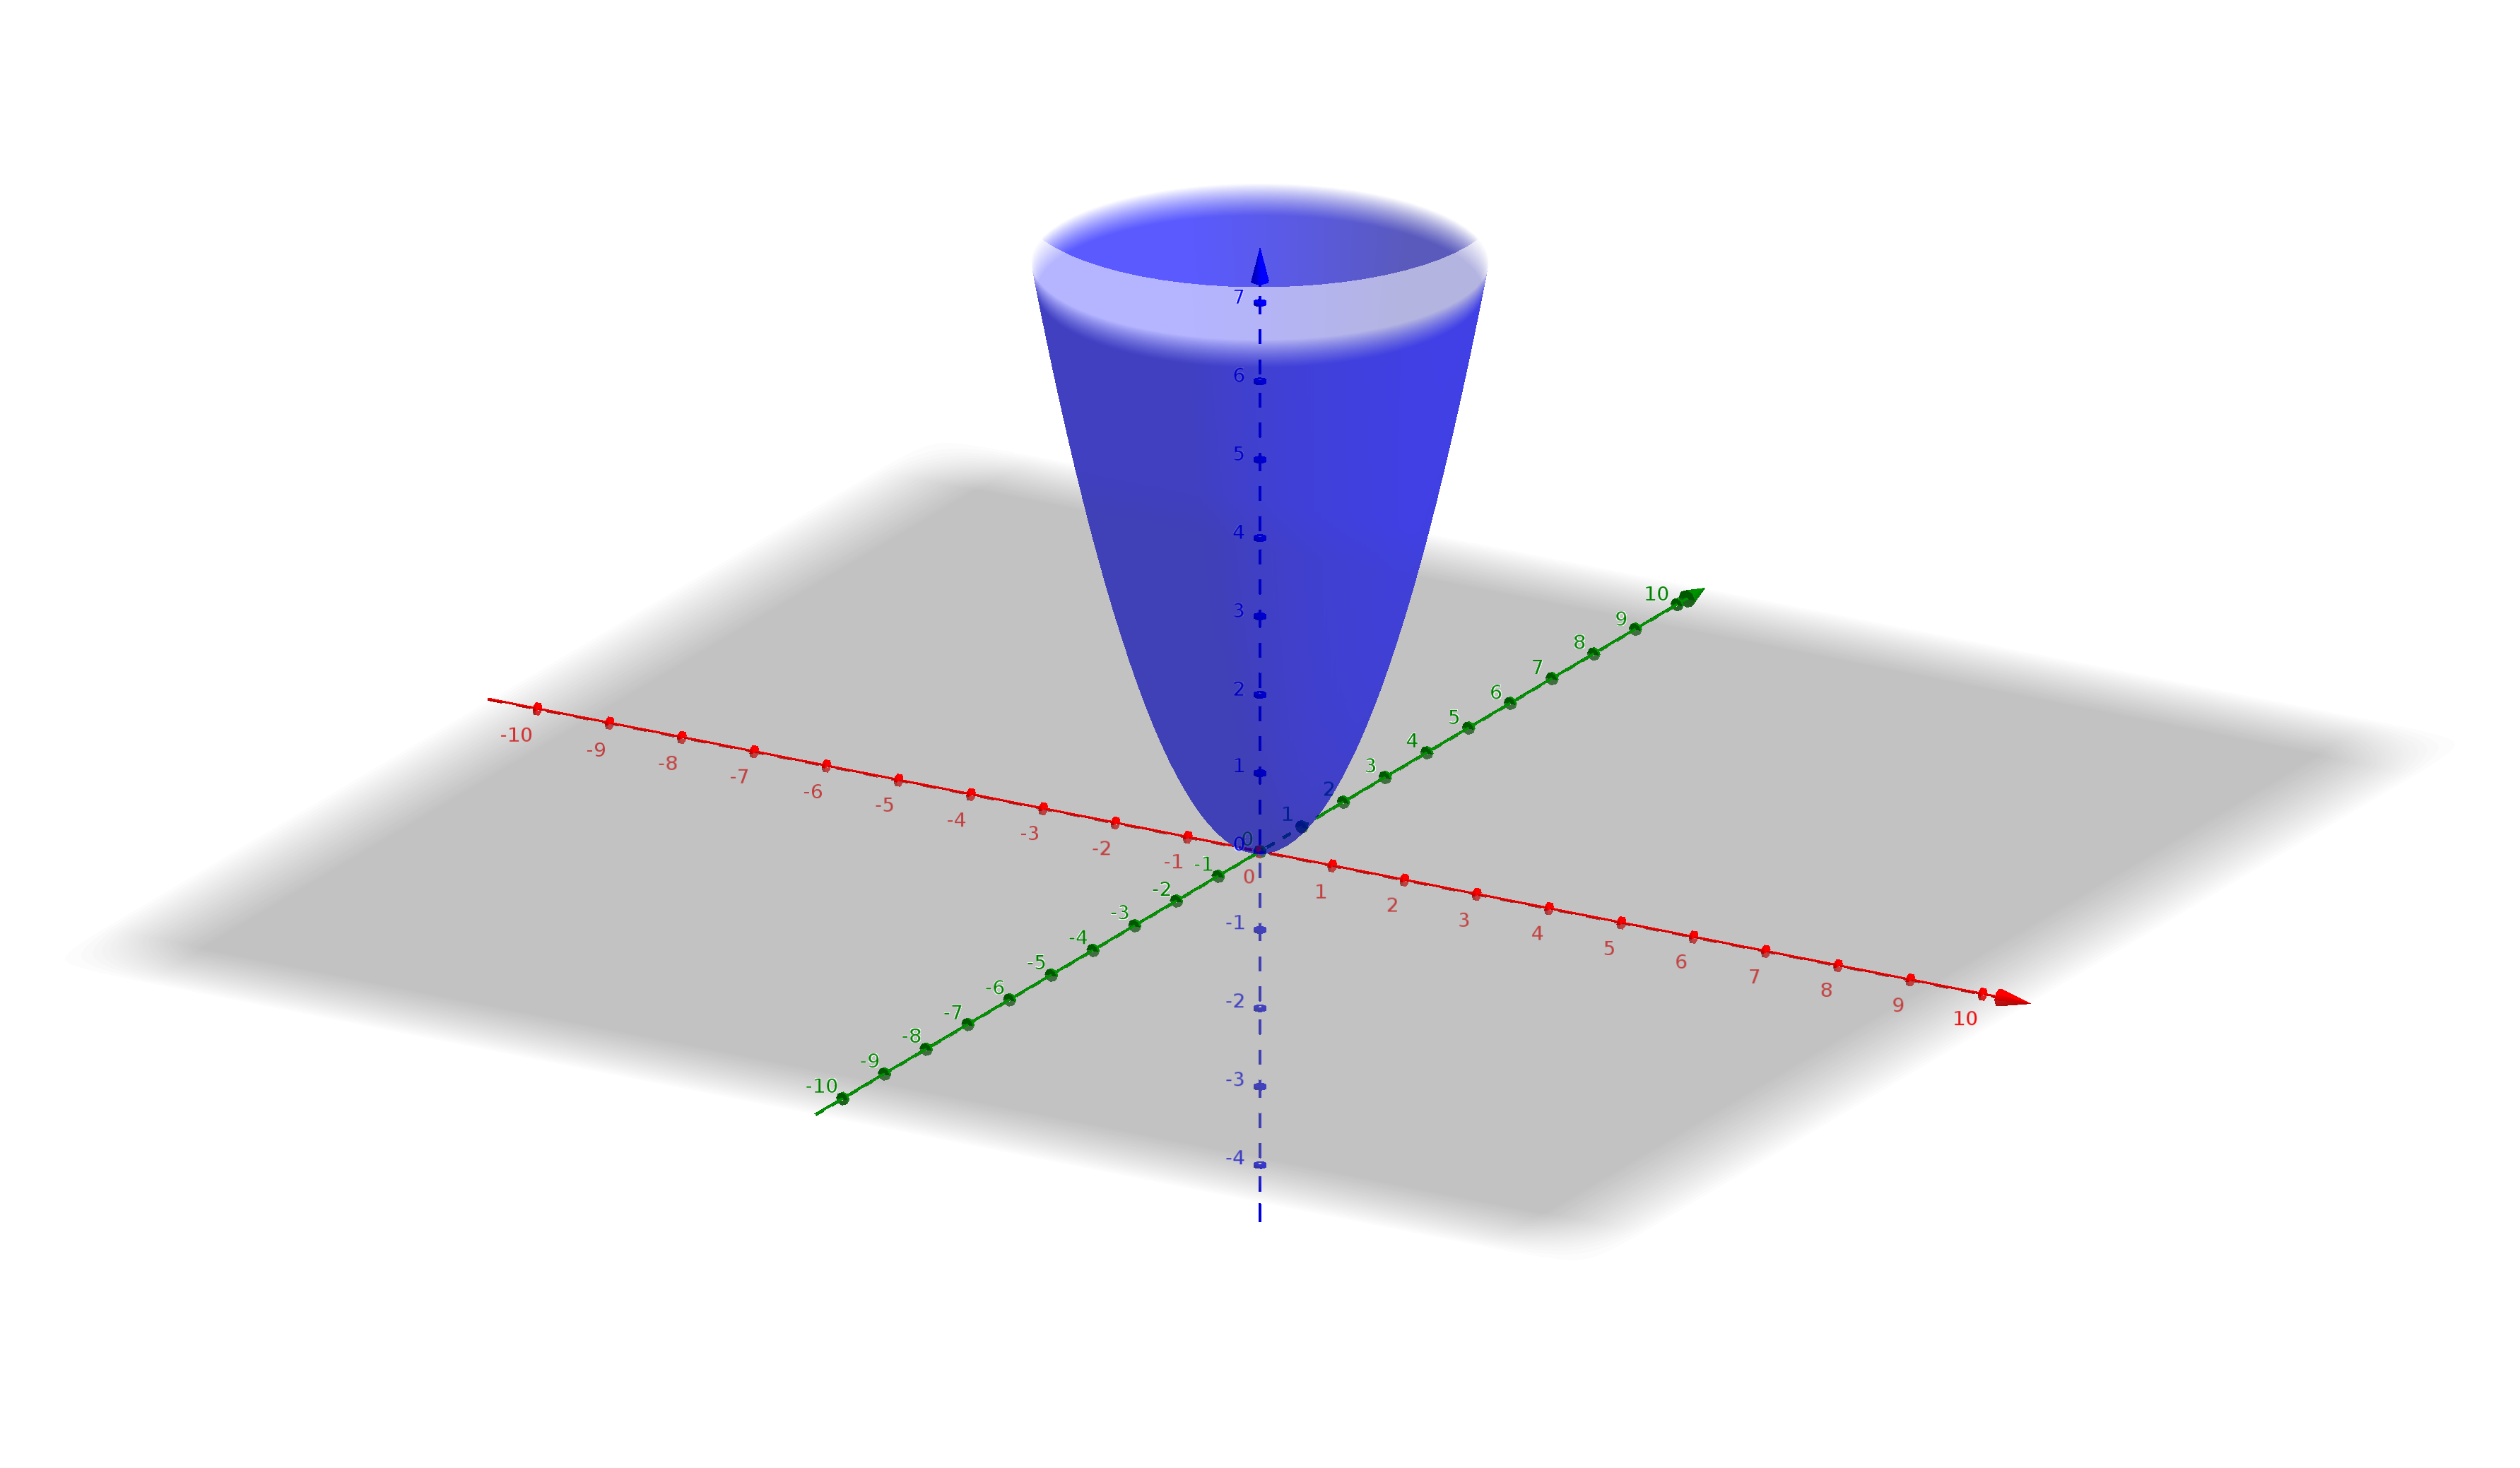
\includegraphics[width=0.5\textwidth]{Paraboloid.png}
    \end{multicols}
    \textbf{The Hyperbolic Paraboloid:}
    \begin{multicols}{2}
        \begin{equation}z=\pm\left(\frac{x^2}{a^2}-\frac{y^2}{b^2}\right)\end{equation}
        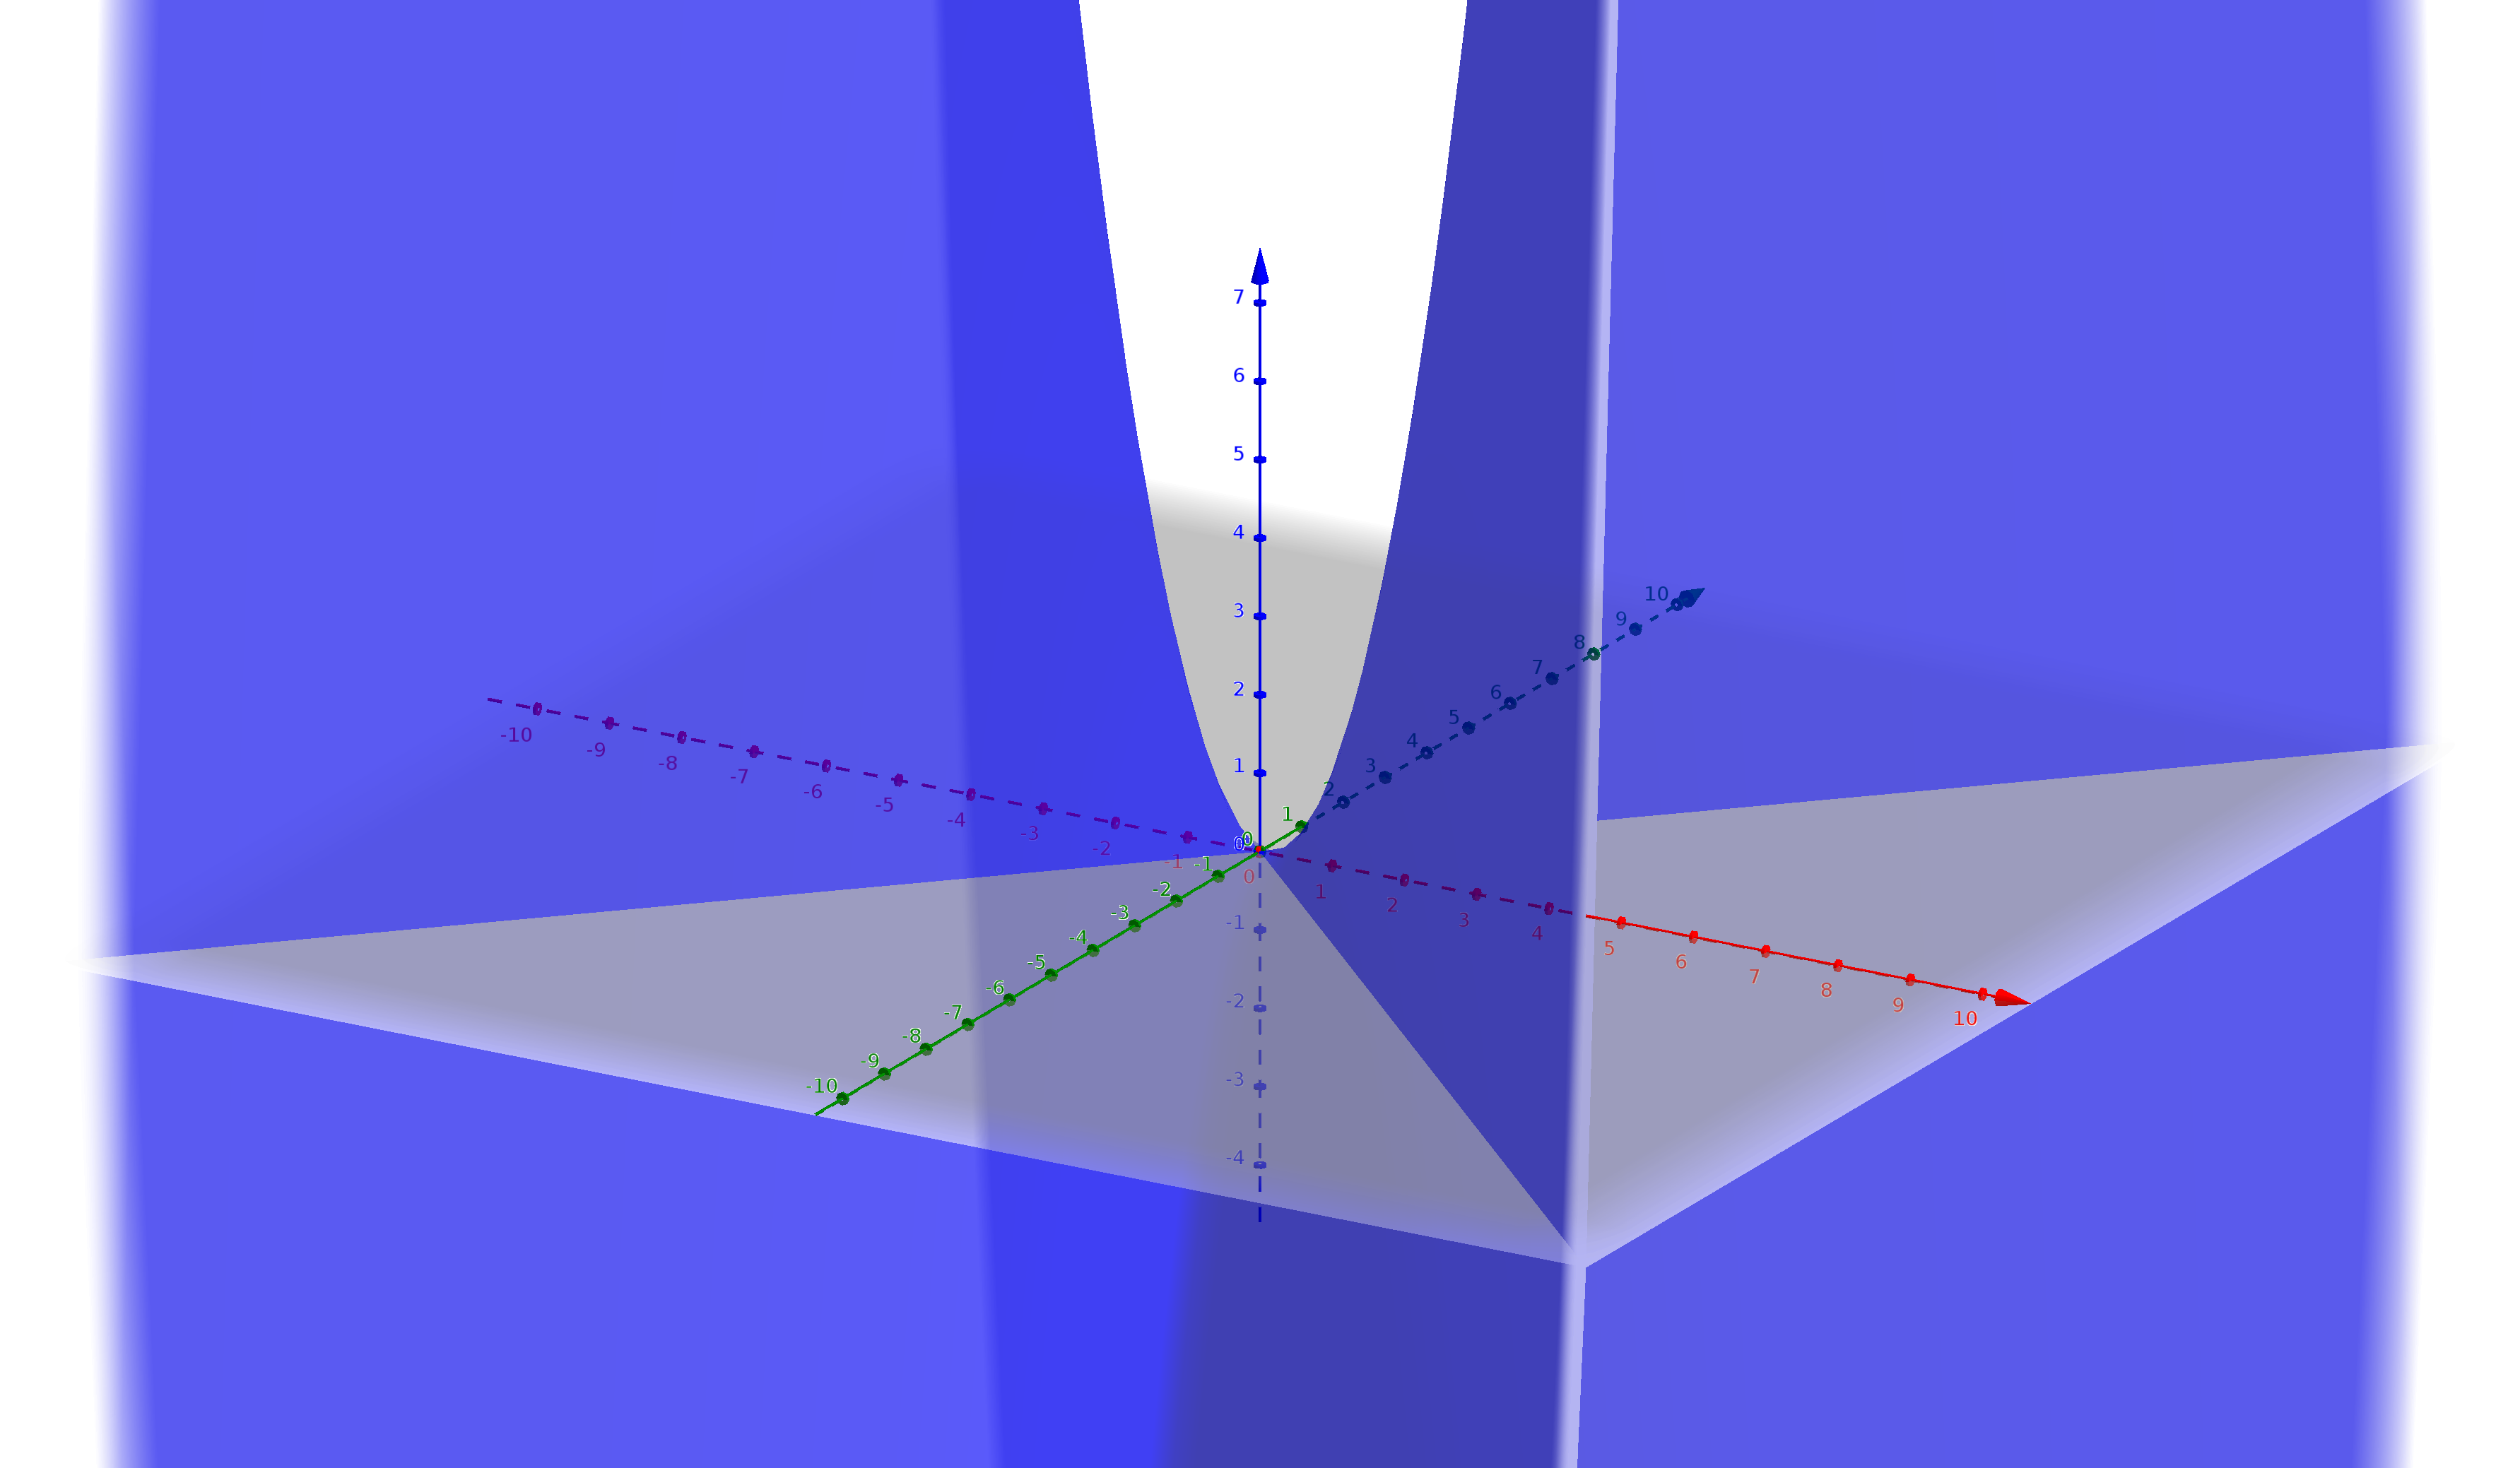
\includegraphics[width=0.5\textwidth]{Hyperbolic_Paraboloid.png}
    \end{multicols}
    Each Paraboloid has vertex at the origin $(0,0,0)$ and axis of symmetry about the z-axis.
    \pagebreak
    \subsubsection{The Hyperboloid Family:}
    \textbf{The Hyperboloid of One Sheet:}
    \begin{multicols}{2}
        \begin{equation}\frac{x^2}{a^2}+\frac{y^2}{b^2}-\frac{z^2}{c^2}=1\end{equation}
        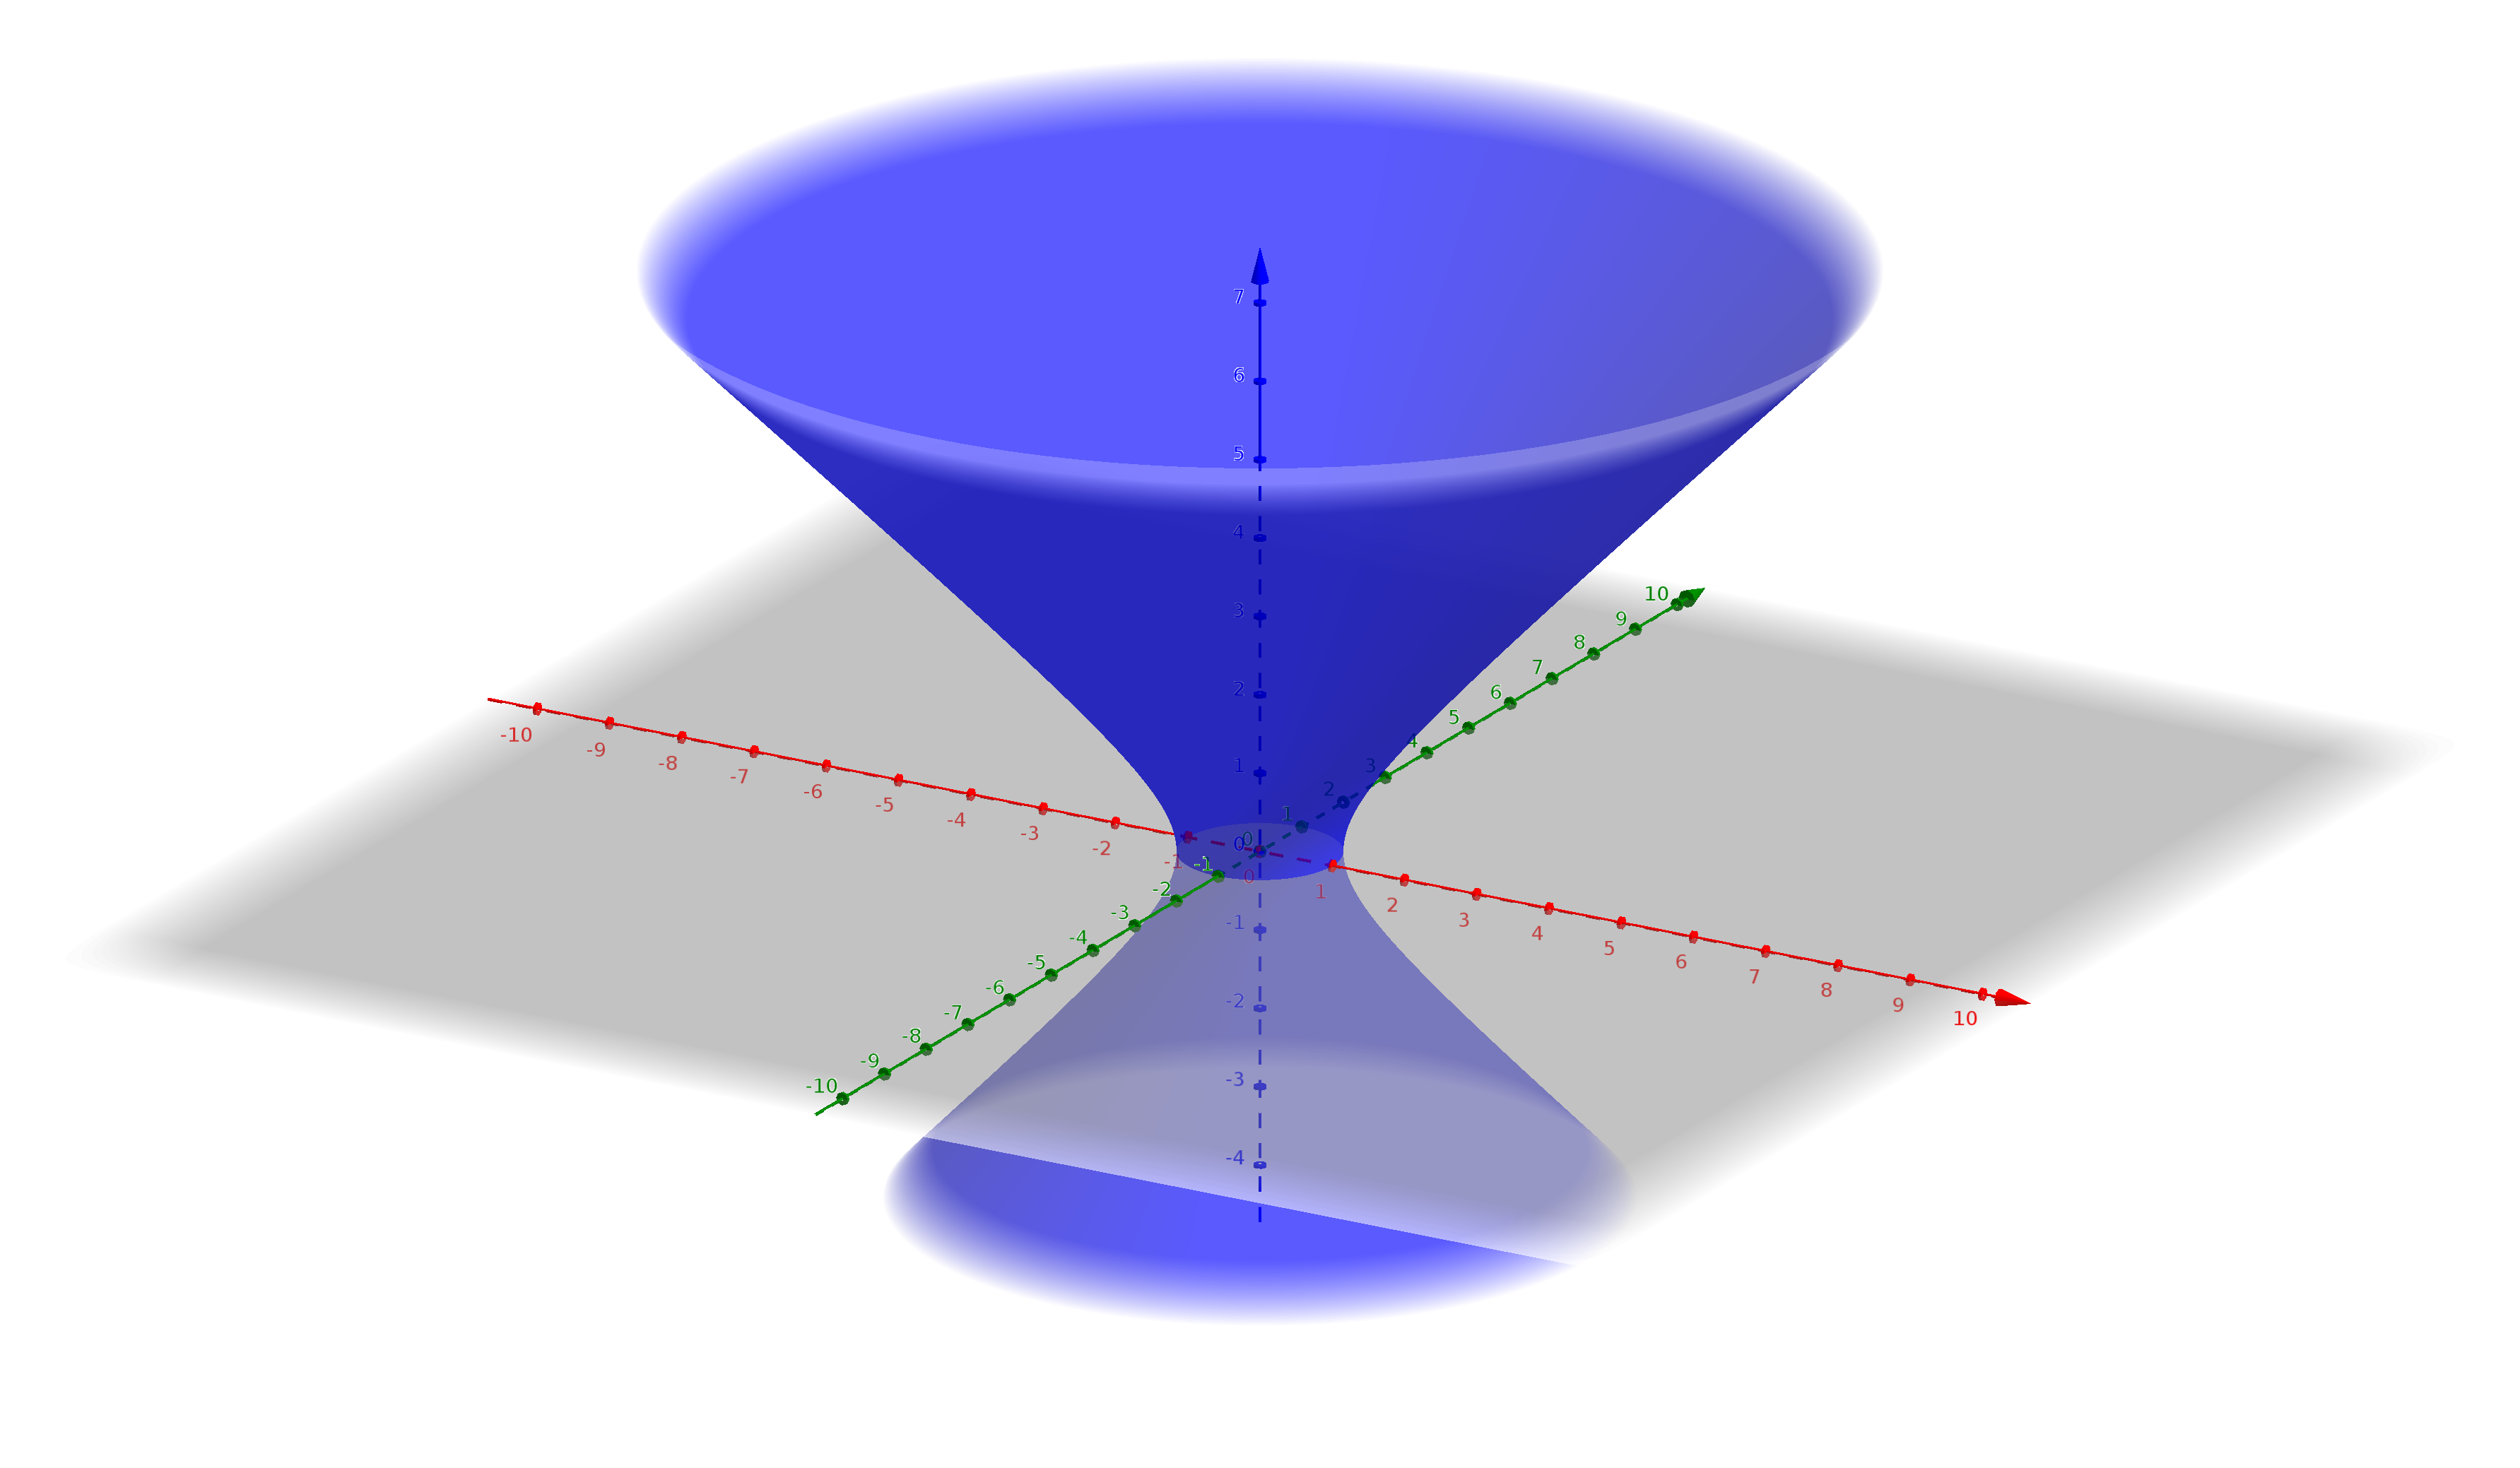
\includegraphics[width=0.5\textwidth]{Hyperboloid1.png}
    \end{multicols}
    
    \textbf{The Hyperboloid of Two Sheets:}
    \begin{multicols}{2}
        \begin{equation}\frac{x^2}{a^2}+\frac{y^2}{b^2}-\frac{z^2}{c^2}=-1\end{equation}
        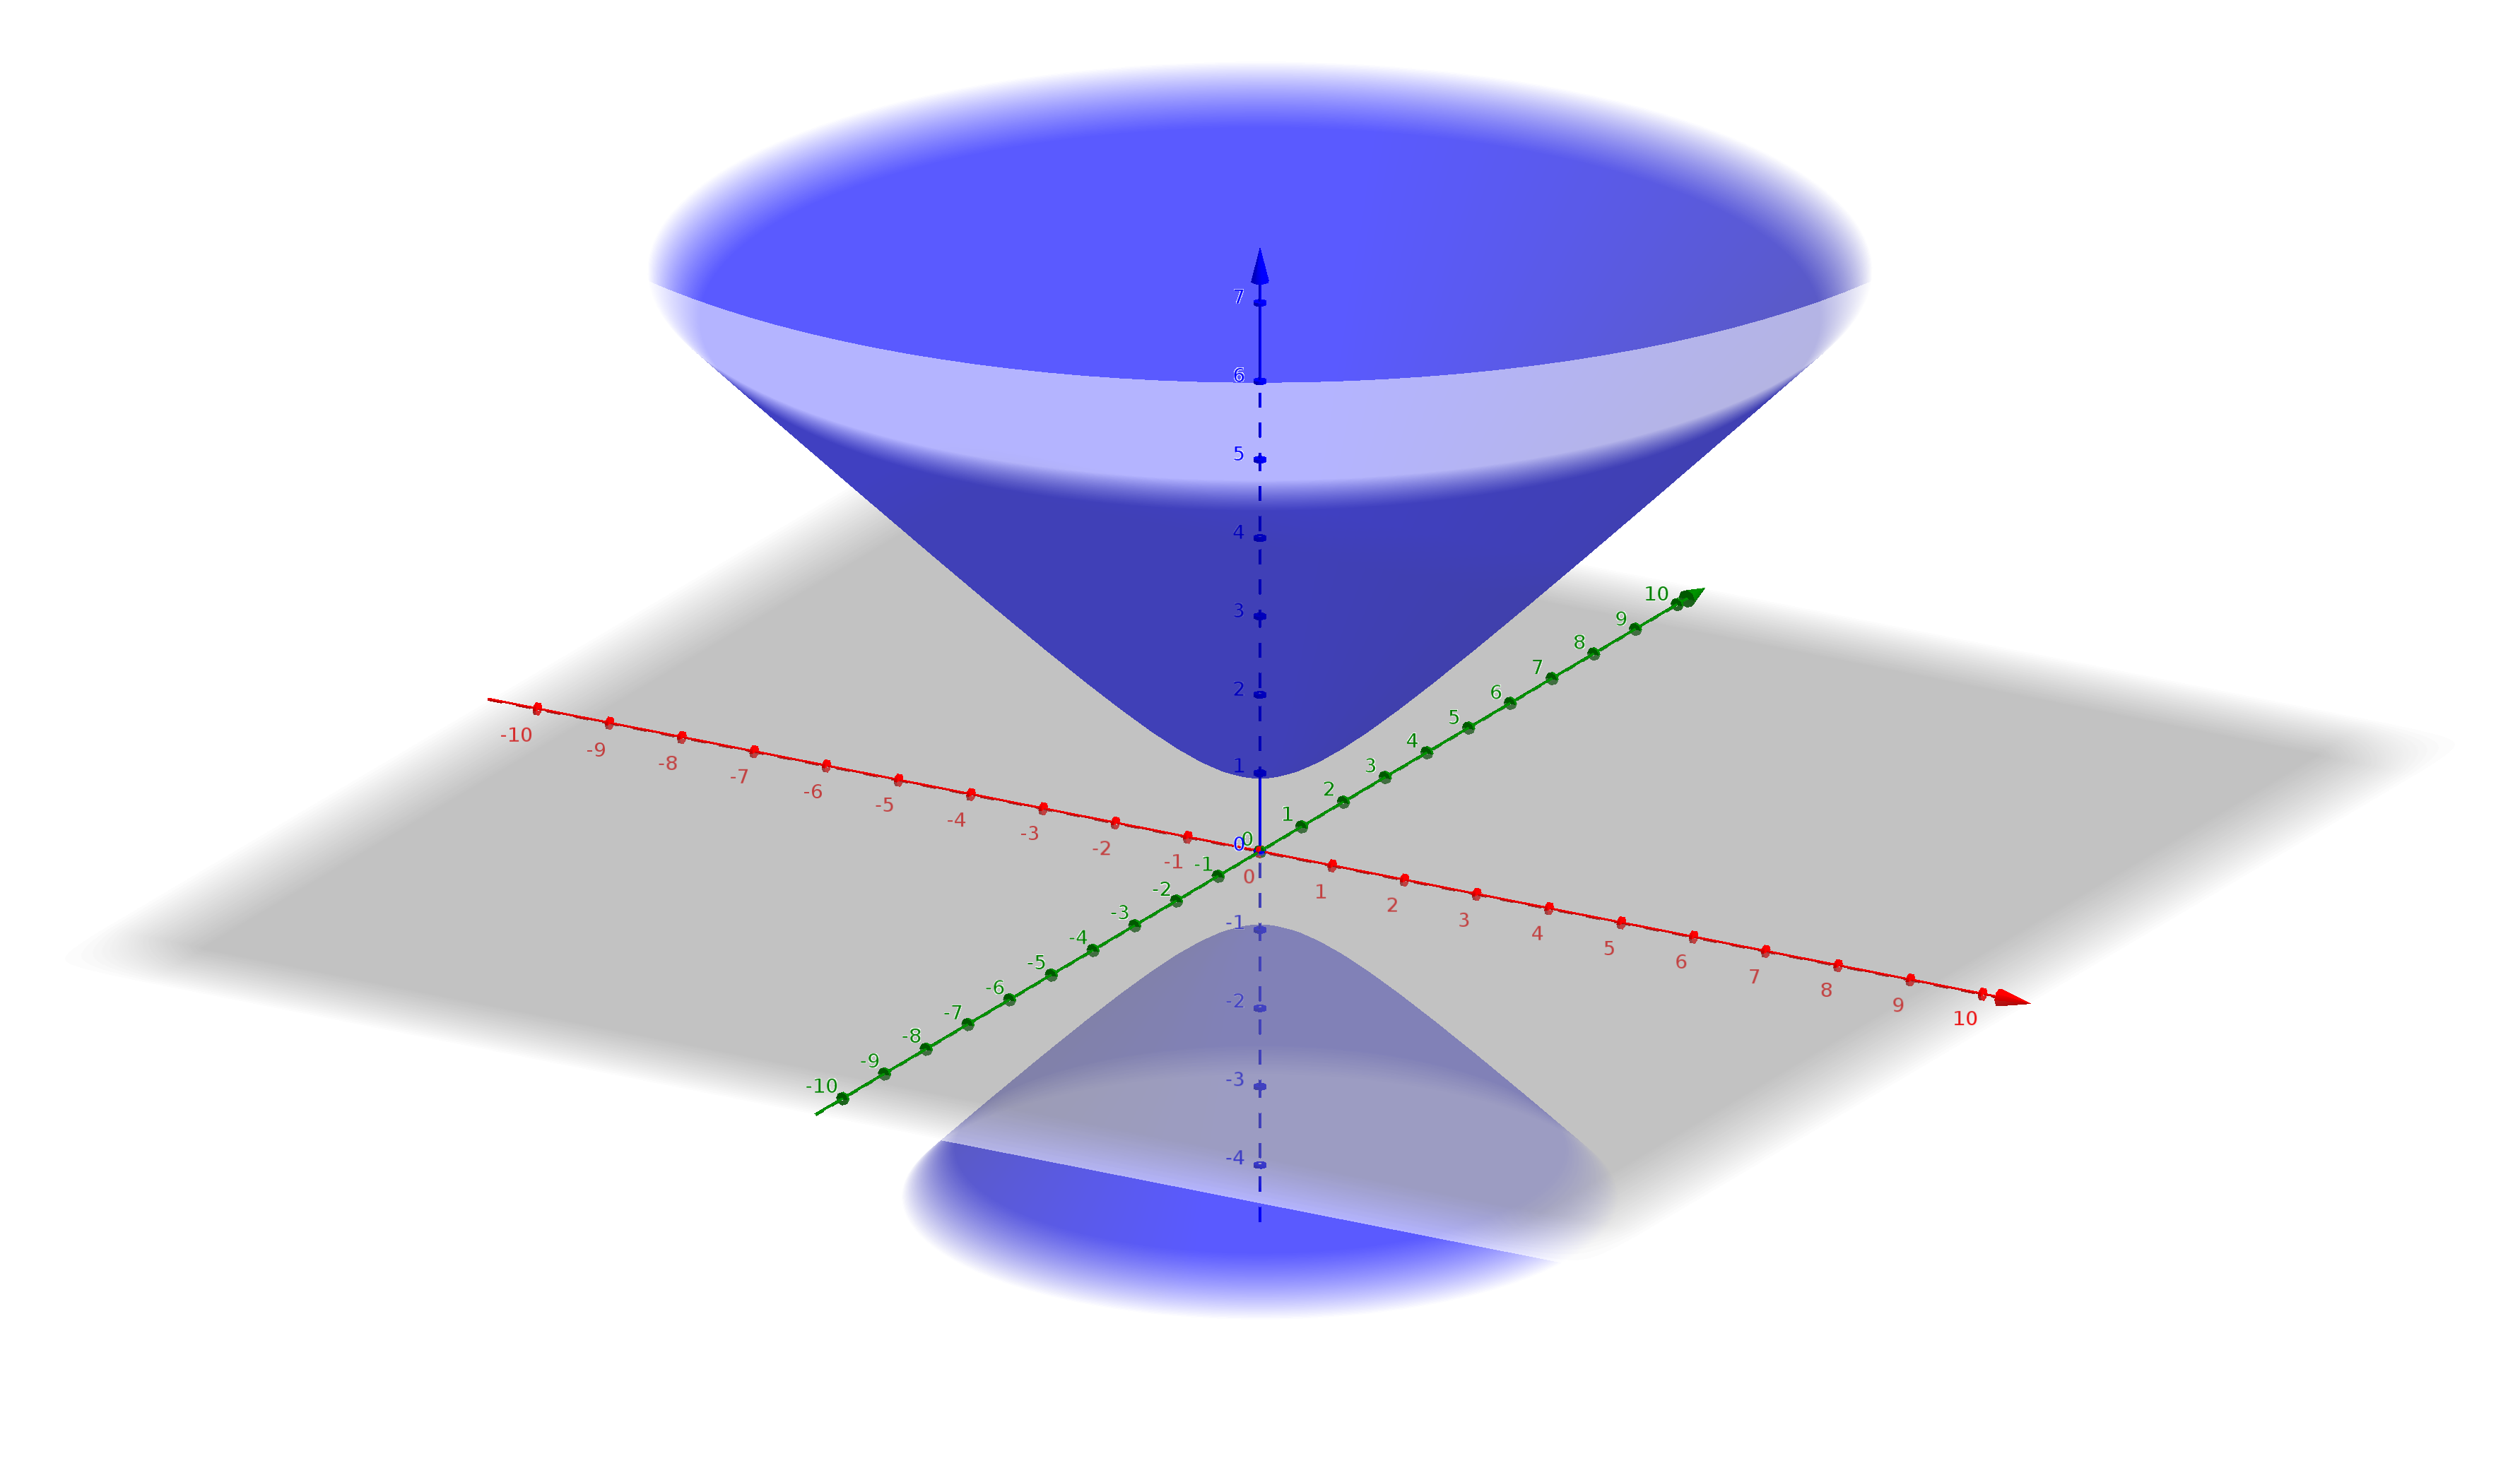
\includegraphics[width=0.5\textwidth]{Hyperboloid2.png}
    \end{multicols}
    
    \textbf{The Cone:}
    
    \begin{multicols}{2}
        \begin{equation}z^2=\frac{x^2}{a^2}+\frac{y^2}{b^2}\end{equation}
        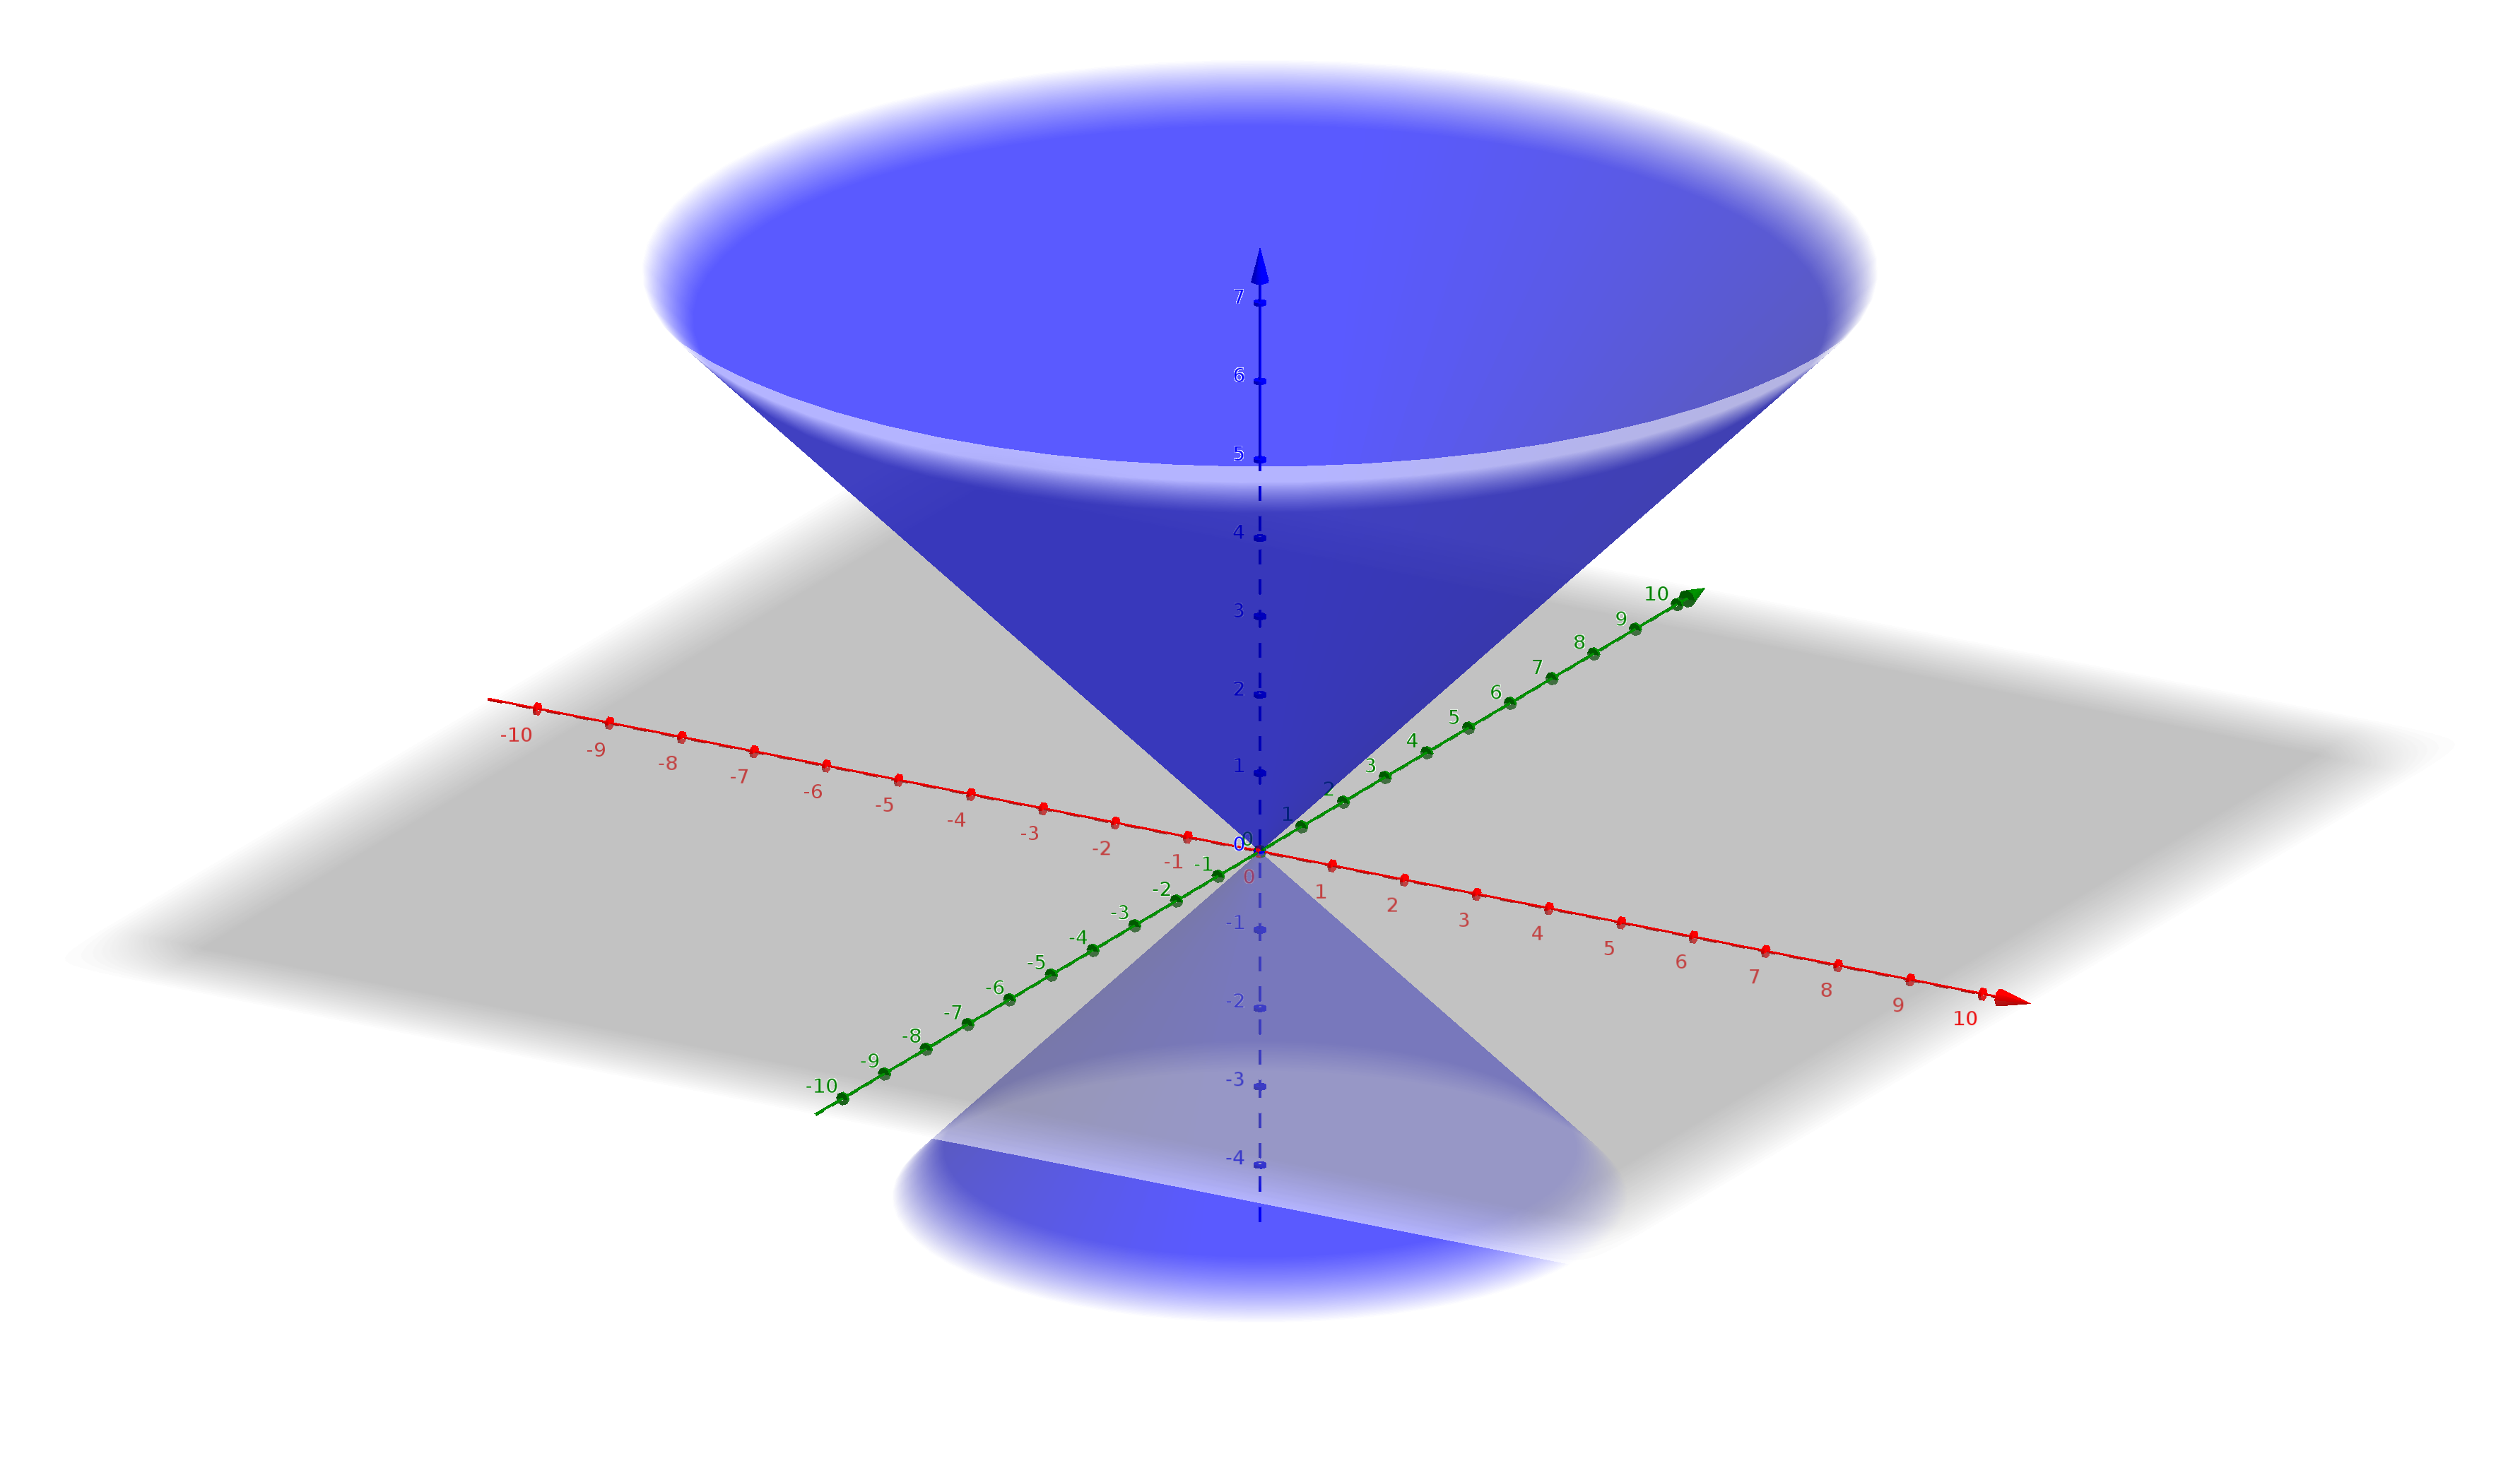
\includegraphics[width=0.5\textwidth]{Cone.png}
    \end{multicols}
    Hyperboloids of one and two sheets have centers about the origin $(0,0,0)$ and a axis of symmetry about the z-axis. If the cone has $a=b$ then it is a circular cone. If we solve the equation of the cone for $z$.
    $$z=\pm\sqrt{\frac{x^2}{a^2}+\frac{y^2}{b^2}}$$
    With the positive being the upper half and the negative being the lower half.\\\\
    If in all eight equations we replace $x$, $y$, and $z$ respectively by $x-h$, $y-k$ and $z-l$, we obtain a translated quadric surface with center or vertex at $(h,k,l)$. The equation of a quadric surface with axis of symmetry being or parallel to the x or y-axis is similar to the z axis.
    \subsection{Special Surfaces:}
    \subsubsection{The Plane:}
    $$Ax+By+Cz=D$$
    where $A$, $B$, $C$, $D$ are real and not all 0. There are 6 special planes.
    \begin{enumerate}
        \item $z=0$ The equation of the $xy$ plane.
        \item $z=l$ A plane parallel to the $xy$ plane $l$ units apart.
        \item $y=0$ The equation of the $xz$ plane.
        \item $y=k$ A plane parallel to the $xz$ plane $k$ units apart.
        \item $x=0$ The equation of the $yz$ plane.
        \item $x=h$ A plane parallel to the $yz$ plane $h$ units apart.
    \end{enumerate}
    \subsubsection{Special Cylinders}
    An equation in $\mathbb{R}^3$ containing only 2 variables is an equation of a cylinder with generators parallel to the missing variable axis. The function $F(x,y)=0$ is a cylinder parallel to the $z$-axis where $F(x,y)=0$ is the boundary of the base of the cylinder.
    \subsection{Functions of two and three independent Variables:}
    \subsubsection{A Function of Two Independent Variables:}
    A function $f$ of two independent variables is a rule that assigns to each permissible ordered pair from a set $D$ in the $xy$-plane, one and only one real number $z$ and is denoted
    $$z=f(x,y)$$
    A function of three or more independent variables is defined similarly.\\\\
    \subsubsection{Domain of a Function of Two Independent Variables:}
    The domain of $z=f(x,y)$ is the set (collection) of all ordered pairs $(x,y)$ such that $f$ is defined and real. The domain of $f$ may be denoted $D$ or $dmf$. The domain for functions of three or more variables is defined similarly.
    \subsubsection{Graph of a Function of Two Independent Variables:}
    First recall the graph of a function of a single variable $y=f(x)$ is: The set of ordered pairs of $(x,f(x))$. The graph of a function of a single variable is referred to as a curve in $\mathbb{R}^2$. Likewise the graph of a function of two independent variables $z=f(x,y)$ is the set of all ordered triples,
    $$(x,y,z)=(x,y,z(f(x,y)))$$
    The graph of $z=f(x,y)$ is referred to as a surface in $\mathbb{R}^3$. Likewise for a function of $n$ variables its graph generates a hypersurface in $\mathbb{R}^{n+1}$\\\\
    \subsubsection{Level Curves and Surfaces of a function of 2 or 3 variables:}
    Let $S$ be the surface given by $z=f(x,y)$. If $z$ is fixed to a constant $z=c$, then the curve $c=f(x,y)$, is a cross section or level curve of $f$ at $z=c$.
    Likewise if we have a hypersurface $w=f(x,y,z)$, $w$ can be fixed as a constant $w=c$ and then $c=f(x,y,z)$ is a level surface in $\mathbb{R}^3$.
    A collection of level curves is known as a contour map.
    \subsection{Partial Derivatives for functions of Several Variables}
    \subsubsection{Partial Derivatives of a function of Two Independent Variables}
    Let $z=f(x,y)$. The partial derivative of $z$ with respect to $x$ is denoted and defined by
    $$\frac{\partial z}{\partial x}=f_x=\lim\limits_{h\rightarrow 0}\frac{f(x+h, y)-f(x,y)}{h}$$
    provided the limit exists.\\
    The partial derivative of $z$ with respect to $y$ is denoted and defined by
    $$\frac{\partial z}{\partial y}=f_y=\lim\limits_{k\rightarrow 0}\frac{f(x, y+k)-f(x,y)}{k}$$
    provided the limit exists. It is evident from the definition that to compute $f_x$ treat $y$ as a constant and differentiate. The partial derivative $f_y$ is computed similarly by holding $x$ constant.
    \subsubsection{Other Notation for Partial Derivatives:}
    Let $z=f(x,y)$. The partial derivative of $f$ may be denoted by
    \begin{enumerate}
        \item $\frac{\partial f}{\partial x}$, $\frac{\partial f}{\partial y}$
        \item $f_x(x,y)$, $f_y(x,y)$
        \item $f_1(x,y)$, $f_2(x,y)$
    \end{enumerate} 
    \subsubsection{Partial Derivatives of functions of $n$ independent variables}
    Let $f(x_1, x_2, \cdots, x_n)$ be a function of $n$ independent variables. The partial derivative of $f$ with respect to $x_i$ where $i\in \mathbb{N},\ i\leq n$ is given by
    $$\frac{\partial f}{\partial x}=\lim\limits_{h\rightarrow 0}\frac{f(x_1, x_2, \cdots, x_i+h, \cdots, x_n)-f(x_1, x_2, \cdots, x_n)}{h}$$
    provided the limit exists.
    \subsubsection{Higher Order Derivatives:}
    Let $z=f(x,y)$. $\frac{\partial z}{\partial x}$ and $\frac{\partial z}{\partial y}$ are called the first order partial derivatives of $f$. The second order partial derivatives are given by
    $$\frac{\partial^2z}{\partial x^2}=f_{xx}=\frac{\partial}{\partial x}\left(\frac{\partial z}{\partial x}\right)$$ 
    $$\frac{\partial^2z}{\partial y^2}=f_{yy}=\frac{\partial}{\partial y}\left(\frac{\partial z}{\partial y}\right)$$
    Mixed Partials
    $$\frac{\partial^2 z}{\partial x\partial y}=f_{yx}=\frac{\partial}{\partial x}\left(\frac{\partial z}{\partial y}\right)$$
    $$\frac{\partial^2 z}{\partial y\partial x}=f_{xy}=\frac{\partial}{\partial y}\left(\frac{\partial z}{\partial x}\right)$$
    The mixed partials are not necessarily equal. Let $z=f(x,y)$. If $f_x$, $f_y$, $f_{xy}$, $f_{yx}$ are all continuous at some point $P$, then the mixed partials exist and are equal at $P$.
    $$\frac{\partial^2 z}{\partial x\partial y}=\frac{\partial^2 z}{\partial y\partial x}$$
    Second order derivatives are defined similarly for functions of more variables. In general for a function of $m$ variables there is $m^n$ $n^{\mathrm{th}}$ order derivatives.
    \subsubsection{The Chain Rule for functions of Several Variables:}
    Let us first recall the chain rule for a single variable function. Let $y=f(x)$ where $x$ is a function of $t$ or $x=x(t)$. Hence $y$ is indirectly a function of $t$, That is $y=y(t)$. To find $\frac{dy}{dt}$ compute,
    $$\frac{dy}{dt}=\frac{df}{dx}\frac{dx}{dt}$$
    Likewise $z=f(x,y)$ where $x$ and $y$ are functions of $t$, or $x=x(t)$, $y=y(t)$. Obviously $z$ is a function of $t$, $z=z(t)$. It can be shown that,
    $$\frac{dz}{dt}=\frac{\partial f}{\partial x}\frac{dx}{dt}+\frac{\partial f}{\partial y}\frac{dy}{dt}$$
    There are endless formula for the chain rule for functions of several variables. Another example is let $z=f(x,y)$ where $x=x(u,v)$ and $y=y(u,v)$. Now $z$ is a function fo $u$ and $v$ and has derivatives
    $$\frac{\partial z}{\partial u}=\frac{\partial z}{\partial x}\frac{\partial x}{\partial u}+\frac{\partial z}{\partial y}\frac{\partial y}{\partial u}$$
    $$\frac{\partial z}{\partial v}=\frac{\partial z}{\partial x}\frac{\partial x}{\partial v}+\frac{\partial z}{\partial y}\frac{\partial y}{\partial v}$$
    \subsection{Tangent Planes and Normal Line to Surface:}
    \subsubsection{Gradient of a Function of Several Variables}
    Let $f(x,y,z)$ be a function of three independent variables $x$, $y$, and $z$, and let $P$ be the point $(x_0, y_0, z_0)$. The gradient of $F$ at $P$ is denoted and defined by
    $$\vec\nabla F=\begin{pmatrix}
        \frac{\partial F}{\partial x}\\
        \frac{\partial F}{\partial y}\\
        \frac{\partial F}{\partial z}
    \end{pmatrix}$$
    \subsubsection{Geometric Interpretation of Gradient}
    Let $S$ be the surface given by the equation $F(x,y,z)=0$ and let $P(x_0, y_0, z_0)$ be a point on the surface. It can be easily verified that any vector orthogonal to the surface at $P$ is $N=\vec \nabla F(P)$. The line through point $P$ orthogonal to the surface is called the normal line to the surface at $P$
    \subsubsection{The Point Normal Form of a Plane}
    The equation of  a plane passing through a point $P(x_0, y_0, z_0)$ with a normal vector $\vec N$ has the equation
    $$\vec N\cdot \vec r=0$$
    where the vector $\vec r$ is given by
    $$\vec r=\begin{pmatrix}
        x-x_0\\
        y-y_0\\
        z-z_0
    \end{pmatrix}$$
    This equation is the point normal form of a plane.
    \subsection{Increments and Decrements:}
    Let $F(x,y)$ be a function of two independent variables $x$, and $y$. Assume that $(x,y)$ has changed from the initial value $(x_0, y_0$ to $(x_1, y_1)$. 
    \subsubsection{Increment or Change in Independent Variables}
    The increment or change in independent variables $x$, $y$ are respectively denoted and defined by
    $$\Delta x=x_1-x_0\text{ and }\Delta y=y_1-y_0$$
    The relative change in the dependent variable is
    $$\Delta=z_1-z_0=F(x_1, y_1)-F(x_0, y_0)$$
    \subsubsection{Differentials of Independent and Dependent Variables}
    The differentials of independent variables $x$ and $y$ are respectively denoted and defined by
    $$\partial x=\Delta x\Rightarrow\partial x=x_1-x_0$$
    $$\partial y=\Delta y\Rightarrow\partial y=y_1-y_0$$
    The differential of the dependent variable is denoted and defined by
    \begin{align*}
        \partial z=\partial F &=\frac{\partial F}{\partial x}\partial x+\frac{\partial F}{\partial x}\partial y\\
        \text{or} &= \frac{\partial F}{\partial x}\Delta x+\frac{\partial F}{\partial x}\Delta y
    \end{align*}
    provided $\frac{\partial F}{\partial x}$ and $\frac{\partial F}{\partial y}$ are continuous.\\\\
    We may think of $\Delta x$ and $\Delta y$ as the error in $x$, and $y$ respectively. $\Delta z$ or $F(x_1, y_1)-F(x_0, y_0)$ is not easy to calculate. However $\partial z$ is much easier to calculate. If $(x_1,y_1)$ is close to $(x_0, y_0)$ then
    $$\Delta F(x_1, y_1)\approx \partial F(x_0, y_0)$$
    \subsubsection{Error Types}
    Assume a certain quantity has changed from $P_0$ to $P$. Then $\Delta P= P-P_0$.
    \begin{enumerate}
        \item Error: $\Delta P=P-P_0$
        \item Absolute Error: $|\Delta P|$
        \item Relative Error: $\frac{\Delta P}{P_0}$
        \item Percentage Error: $\frac{\Delta P}{P_0}\times 100\% $ 
    \end{enumerate}
    \subsection{The Laplace Equation in $\mathbb{R}^2$ and $\mathbb{R}^3$}
    The laplace equation in $\mathbb{R}^3$ is given by
    $$\nabla^2u=\frac{\partial^2u}{\partial x^2}+\frac{\partial^2 u}{\partial y^2}+\frac{\partial^2 u}{\partial z^2}=0$$
    An equation $u$ satisfying the laplace equation is called a harmonic function.
    \subsection{Linearization of a function of several variables}
    Let  $z=f(x,y)$ and let $P(x_0, y_0)$ be a given point. The linearization of $f(x,y)$ at a point $P(x_0, y_0)$ is denoted and defined by
    $$L(x,y)=f(x_0,y_0)+f_x(x_0, y_0)(x-x_0)+f_y(x_0, y_0)(y-y_0)$$
    \subsection{Directional Derivatives of functions of several variables}
    Let $f(x,y,z)$ be a function of three independent variables $x$, $y$, and $z$, and let $\vec u=\begin{pmatrix}a\\b\\c\end{pmatrix}$ be a unit vector in the direction from the point $P(x_0, y_0, z_0)$ to an arbitrary point $Q(x,y,z)$. The vector $\vec u$ is defined
    $$\vec u=\frac{\vec{PQ}}{||\vec {PQ}||}=\begin{pmatrix}a\\b\\c\end{pmatrix}$$
    Let $s=||\vec{PQ}||$. Therefore the components of $\vec u$ can be written
    \begin{align}
        as&=x-x_0\label{a}\\
        bs&=y-y_0\label{b}\\
        cs&=z-z_0\label{c}
    \end{align}
    Now let $w=f(x,y,z)$ where $x=x_0+as$, $y=y_0+bs$, $z=z_0+cs$. Hence $w$ is a function of $s$. By the chain rule
    $$\frac{dw}{ds}=f_x(x,y,z)a+f_y(x,y,z)b+f_z(x,y,z)c$$
    and evaluate $\frac{dw}{ds}$ at $s=0$. Recall \eqref{a}, \eqref{b}, and \eqref{c}. If $s=0$ is Substituted into \eqref{a}, \eqref{b}, and \eqref{c} it is easily shown that $x=x_0$, $y=y_0$, and $z=z_0$. Therefore
    \begin{equation}\label{dwds}
        \bigg. \frac{dw}{ds}\bigg|_{s=0}=f_x(x_0,y_0,z_0)a+f_y(x_0,y_0,z_0)b+f_z(x_0,y_0,z_0)c
    \end{equation}
    The result \eqref{dwds} can berepresented as a dot product of two vectors,
    \begin{align*}
        \frac{dw}{ds}&=\begin{pmatrix}f_x(x_0, y_0, z_0)\\f_y(x_0, y_0, z_0)\\f_z(x_0, y_0, z_0)\end{pmatrix}\cdot\begin{pmatrix}a\\b\\c\end{pmatrix}\\
        &=\vec\nabla f(P)\cdot \vec u
    \end{align*}
    The above result is the directional derivative. The directional derivative of the function $f(x,y,z)$ at the point $P(x_0,y_0,z_0)$ in the direction of the unit vector $\vec u$ is denoted and defined by
    \begin{align*}
        D_{\vec u}f(P)&=\bigg. \frac{dw}{ds}\bigg|_{s=0}\\
        D_{\vec u}f(P)&=\vec\nabla f(P)\cdot \vec u
    \end{align*}
    The directional derivative $D_{\vec u}f(P)$ is the rate of change of the function $f$ at the point $P$ in the direction of the unit vector $\vec u$.
    \subsubsection{Maximum and Minimum Rates}
    Recall the angle $\theta$ between the vectors $\vec a$ and $\vec b$ is given by
    $$\cos\theta=\frac{\vec a\cdot \vec b}{||\vec a||\, ||\vec b||}$$
    Now let $\theta$ be the angle between $\vec\nabla f(P)$ and the unit vector $\vec u$
    $$\therefore \vec\nabla f(P)\cdot \vec u=||\vec\nabla f(P)||\,||\vec u||\cos\theta$$
    but $\vec u$ is a unit vector and $||\vec u||=1$
    $$\vec\nabla f(P)\cdot \vec u=||\vec\nabla f(P)||\cos\theta$$
    $$\therefore D_{\vec u}f(P)= ||\vec\nabla f(P)||\cos\theta$$
    The directional derivative has extreme values when $\cos\theta=\pm1$. $D_{\vec u}f(P)$ has an absolute maximum $||\vec\nabla f(P)||$ when $\theta=0$, and $\vec u$ must be in the direction of $\vec n_1=\frac{\vec\nabla f(P)}{||\vec\nabla f(P)||}$. $D_{\vec u}$ has an absolute minimum $-||\vec\nabla f(P)||$ when $\theta=\pi$ and must be in the direction of $\vec n_2=-\frac{\vec\nabla f(P)}{||\vec\nabla f(P)||}$.
    \subsection{Implicit Differentiation}
    \subsubsection{The Jacobian Determinant}
    The jacobian of 2 functions $F$ and $G$ with respect to the variables $x$ and $y$ is denoted and defined by
    $$J=\frac{\partial(F, G)}{\partial(x, y)}=\begin{vmatrix}
        F_x& F_y\\
        G_x& G_y
    \end{vmatrix}$$
    Likewise the Jacobian of $n$ functions $f_1,\ f_2,\ f_3,\cdots f_n$ with respect to the n variables $x_1,\ x_2,\cdots x_n$ is given by
    $$J=\frac{\partial(f_1, f_2,\cdots, f_n)}{\partial(x_1, x_2,\cdots, x_n)}=\begin{vmatrix}
        \frac{\partial f_1}{\partial x_1} & \frac{\partial f_1}{\partial x_2} & \cdots& \frac{\partial f_1}{\partial x_n}\\
        \frac{\partial f_2}{\partial x_1}&\frac{\partial f_2}{\partial x_2} & \cdots& \frac{\partial f_2}{\partial x_n}\\
        \vdots& \vdots&\ddots & \vdots\\
        \frac{\partial f_n}{\partial x_1}& \frac{\partial f_n}{\partial x_2}& \cdots&\frac{\partial f_n}{\partial x_n} \\
    \end{vmatrix}$$
    The Jacobian of one function $f$ with respect to the variable $x$ is simply $\frac{df}{dx}$
    \subsubsection{Implicit Differentiation}
    Consider a non-linear system that consists of $m$ equations in $n$ variables, where $m\leq n$. Under certain conditions, we may be able to solve for $m$ variables as functions of the remaining $n-m$ variables. For instance consider a system of one non-linear equation in three variables,
    $$F(x,y,z)=0$$
    There are three possible ways to solve this system. It can be solved with $x$ as a function of $y$, and $z$; $y$ as a function of $x$, and $z$; or $z$ as a function of $x$ and $y$. Consider a system of two equations in 5 variables say 
    $$\left\{\begin{array}{lr}
        F(x,y,z,u,v)=0\\
        G(x,y,z,u,v)=0
    \end{array}\right.$$
    There are 10 possible choices of systems to solve for. If we wanted to find $\frac{\partial u}{\partial z}$ where $u=u(x,y,z)$ then it is denoted
    $$\left(\frac{\partial u}{\partial z}\right)_{x,y}$$
    This denotes that $x$,$y$,$z$ are the independent variables and that $u$, and $v$ depend on $x$, $y$, and $z$.
    \subsubsection{A formula for Implicit Integration:}
    Consider a non-linear system of two equations in four variables
    $$\left\{\begin{array}{lr}
        F(x,y,u,v)=0\\
        G(x,y,u,v)=0
    \end{array}\right.$$
    Assume that $u$ and $v$ depend on $x$, and $y$. The system has a condition of solvability and solutions $\frac{\partial u}{\partial x}$, $\frac{\partial u}{\partial y}$, $\frac{\partial v}{\partial x}$, and $\frac{\partial v}{\partial y}$. Let $w=F(x,y,u,v)=0$ where $u=u(x,y)$, $v=v(x,y)$ hence $w=w(x,y)$. By the chain rule
    $$\frac{\partial w}{\partial x}=\frac{\partial F}{\partial x}+\frac{\partial F}{\partial u}\frac{\partial u}{\partial x}+\frac{\partial F}{\partial v}\frac{\partial v}{\partial x}$$
    but with $w=0$ the following is obtained 
    \begin{equation}\label{Fpart}
        -\frac{\partial F}{\partial x}=\frac{\partial F}{\partial u}\frac{\partial u}{\partial x}+\frac{\partial F}{\partial v}\frac{\partial v}{\partial x}
    \end{equation}
    similarly for $G$
    \begin{equation}\label{Gpart}
        -\frac{\partial G}{\partial x}=\frac{\partial G}{\partial u}\frac{\partial u}{\partial x}+\frac{\partial G}{\partial v}\frac{\partial v}{\partial x}
    \end{equation}
    The equation \eqref{Fpart} and \eqref{Gpart} are linear systems in $\frac{\partial u}{\partial x}$ and $\frac{\partial v}{\partial x}$. By Cramer's rule
    \begin{align*}
        \frac{\partial u}{\partial x}=\frac{\begin{vmatrix}
            -\frac{\partial F}{\partial x} & \frac{\partial F}{\partial v}\\
            -\frac{\partial G}{\partial x} & \frac{\partial G}{\partial v}
        \end{vmatrix}}{\begin{vmatrix}
            \frac{\partial F}{\partial u} & \frac{\partial F}{\partial v}\\
            \frac{\partial G}{\partial u} & \frac{\partial G}{\partial v}
        \end{vmatrix}} &&
        \frac{\partial v}{\partial x}=\frac{\begin{vmatrix}
            \frac{\partial F}{\partial u} & -\frac{\partial F}{\partial x}\\
            \frac{\partial G}{\partial u} & -\frac{\partial G}{\partial x}
        \end{vmatrix}}{\begin{vmatrix}
            \frac{\partial F}{\partial u} & \frac{\partial F}{\partial v}\\
            \frac{\partial G}{\partial u} & \frac{\partial G}{\partial v}
        \end{vmatrix}}
    \end{align*}
    Using the Jacobian the following is obtained,
    \begin{align*}
        \frac{\partial u}{\partial x}=-\frac{\frac{\partial(F, G)}{\partial (x, v)}}{\frac{\partial(F, G)}{\partial (u, v)}} &&
        \frac{\partial v}{\partial x}=-\frac{\frac{\partial(F, G)}{\partial (u, x)}}{\frac{\partial(F, G)}{\partial (u, v)}}
    \end{align*}
    provided the denominator $\frac{\partial(F, G)}{\partial (u, v)}\neq 0$. $\frac{\partial u}{\partial y}$ and $\frac{\partial v}{\partial y}$. If there is a non linear system
    $$F(x,y,z)=0$$
    that can be solved for $y$ as a function of $x$ and $z$, then
    \begin{align*}
        \frac{\partial y}{\partial x}=-\frac{F_x}{F_y} && \frac{\partial y}{\partial z}=-\frac{F_z}{F_y}
    \end{align*}
    provided $F_y\neq 0$. 
    \pagebreak
    \section{Double and Triple Integration}
    \subsection{Notation for a Double Integral}
    The double integral of a function $f(x,y)$ over a closed region $D$ in the $xy$-plane (or $\mathbb{R}^2$) is denoted 
    $$\iint\limits_D f(x,y)\, dA$$
    where $dA$ is an element of area and is given by
    $$dA=dx\, dy=dy\, dx$$
    \subsection{Notation for a Triple Integral}
    The triple integral of $f(x,y,z)$ over a closed region $E$ in $xyz$-space (or $\mathbb{R}^3$) is denoted by
    $$\iiint\limits_E f(x,y,z)\, dV$$
    where $dV$ is an element of volume and is given by
    $$dV=dx\, dy\, dz$$
    \subsection{Types of regions in $\mathbb{R}^2$}
    \subsubsection{The $y$-simple Region:}
    A region $D$ is called a $y$-simple region if its bounded from the bottom and top by the continuous curves $y=g(x)$ and $y=h(x)$ respectively and is bound from the left and right by the vertical lines $x=a$ and $x=b$ respectively as shown. A $y$-simple region may be sliced vertically and hence may be described by the pair of inequalities,
    $$D=\left\{\begin{array}{lr}
        a\leq x\leq b\\
        g(x)\leq y \leq h(x)
    \end{array}\right.$$
    \subsubsection{The $x$-simple Region:}
    A region $D$ is called a $x$-simple region if its bounded from the bottom and top by the horizontal lines $y=c$ and $y=d$ respectively and is bound from the left and right by the continuous curves $x=p(y)$ and $x=q(y)$ respectively as shown. A $x$-simple region may be sliced vertically and hence may be described by the pair of inequalities,
    $$D=\left\{\begin{array}{lr}
        p(y)\leq x\leq q(y)\\
        c\leq y \leq d
    \end{array}\right.$$
    \begin{figure}[th!]
        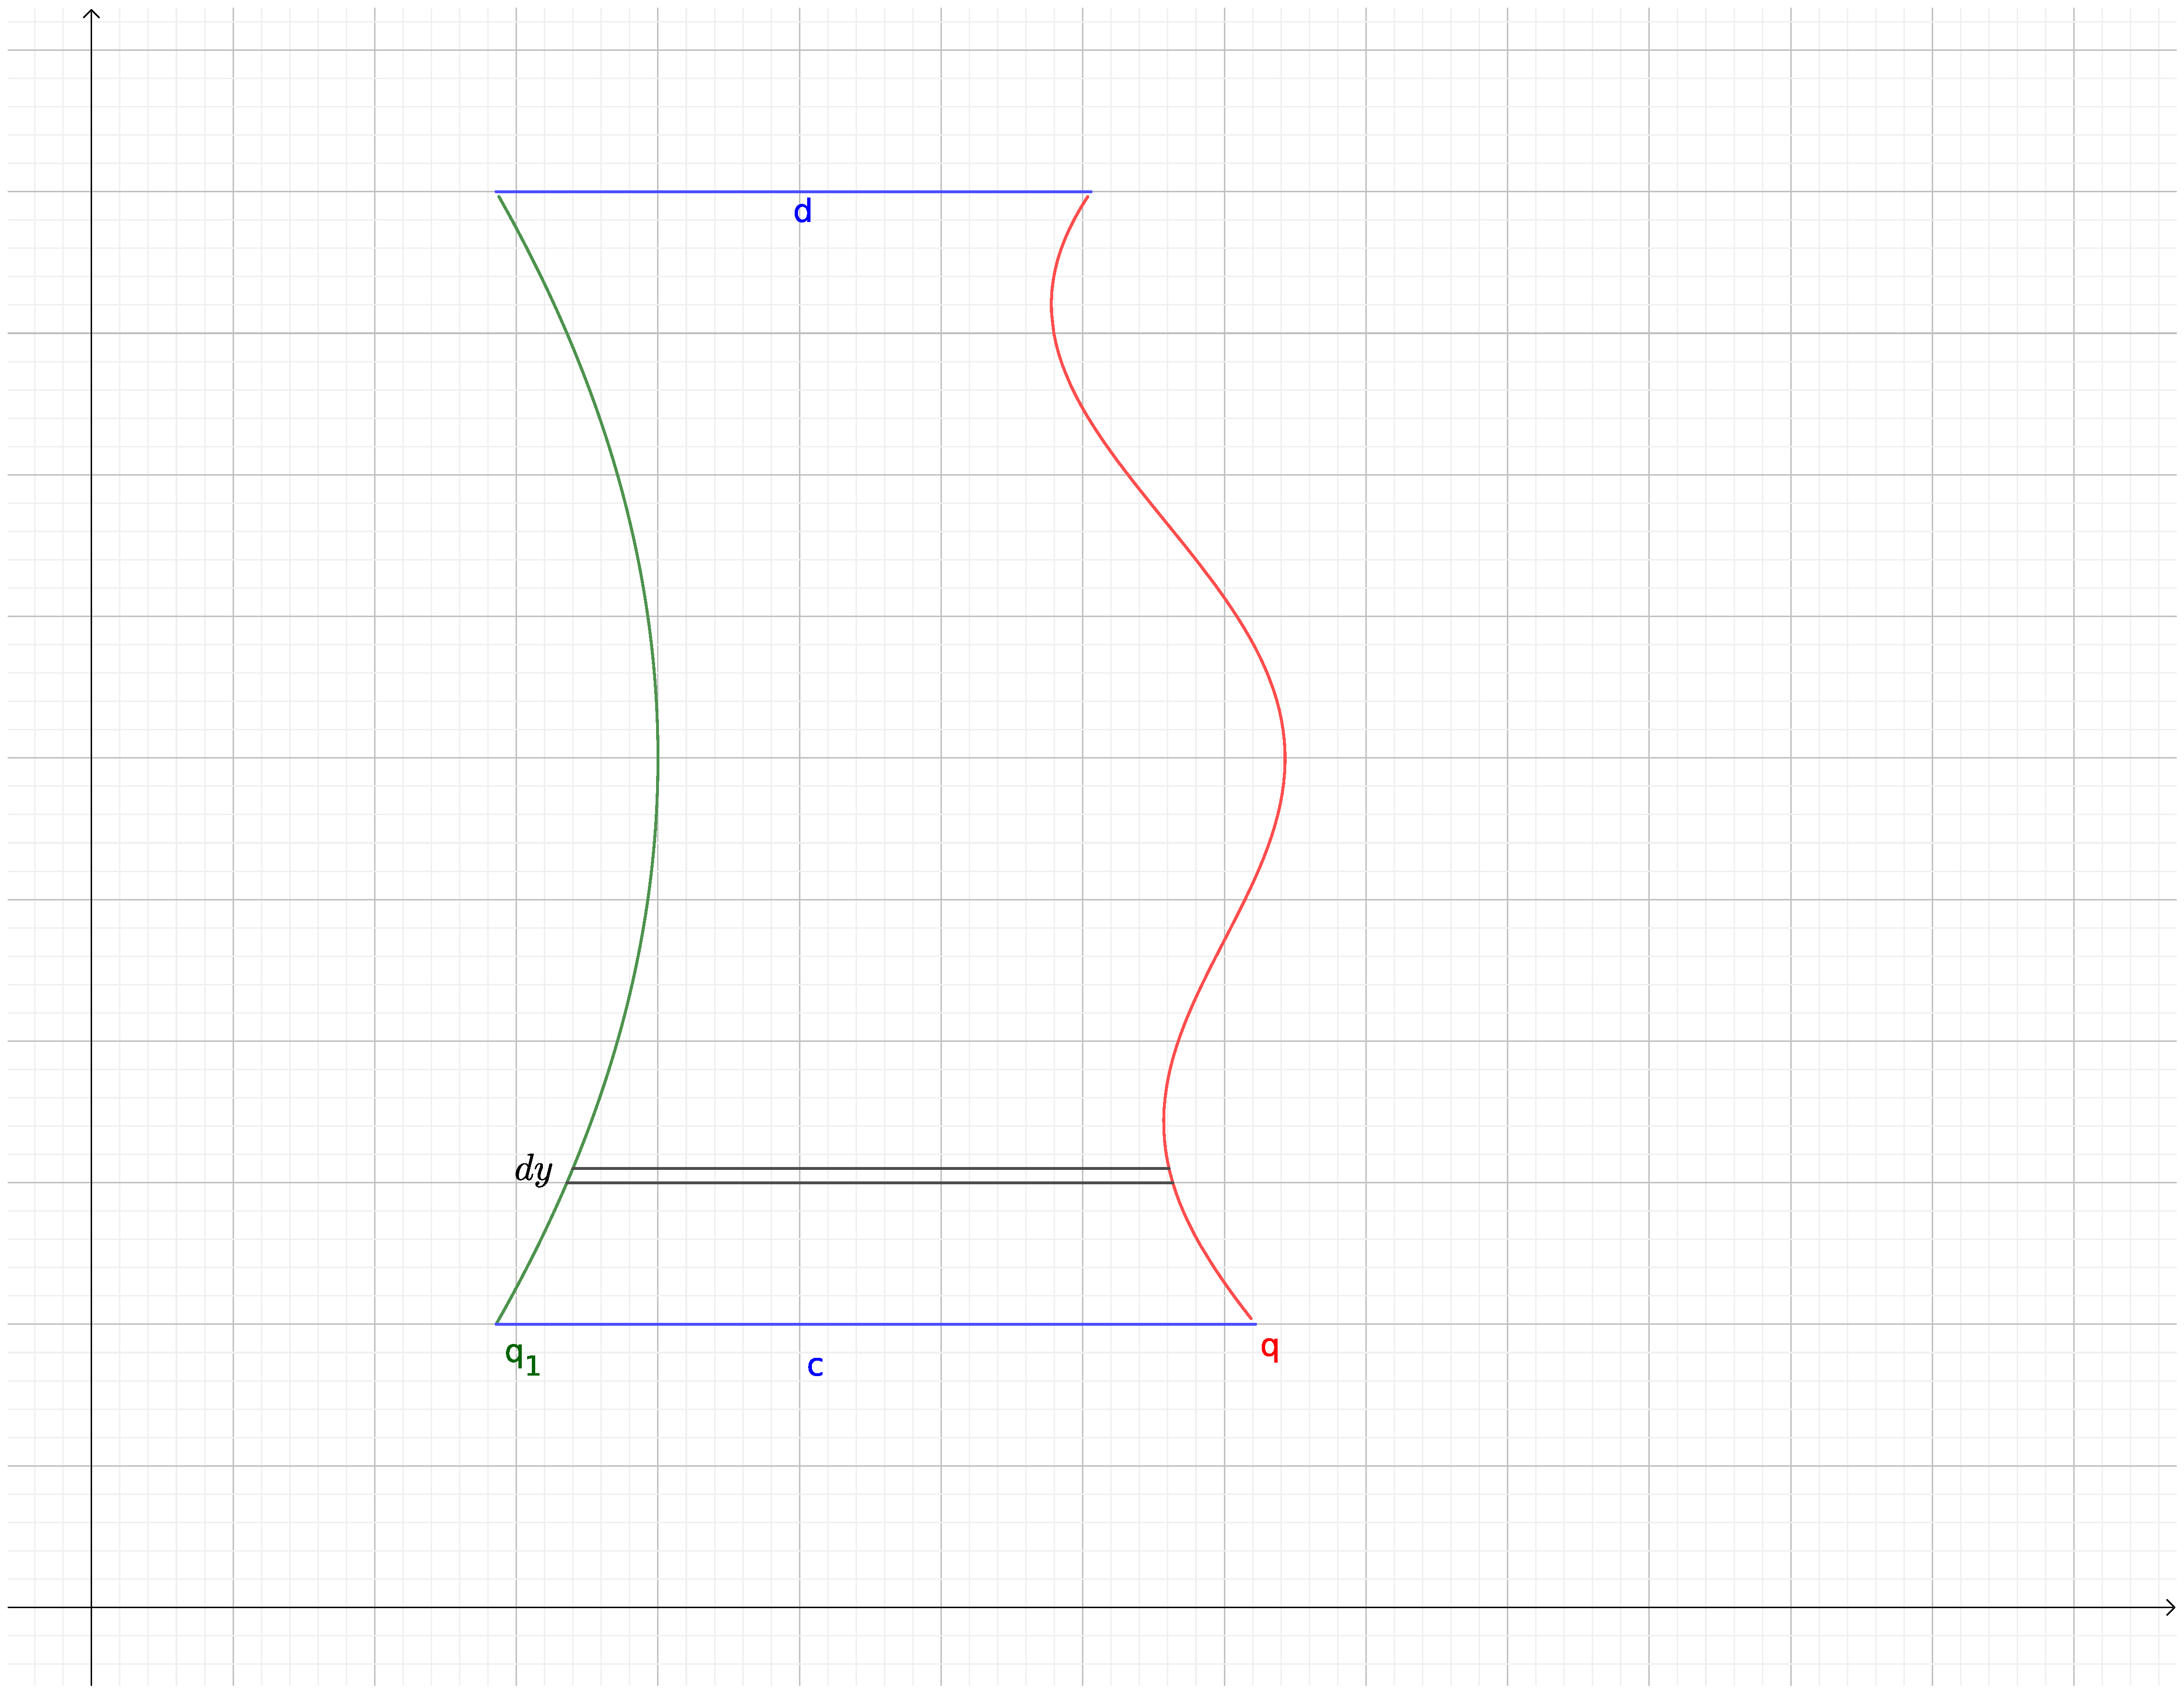
\includegraphics[width=0.45\textwidth]{x-simple.eps}
        \hspace{0.09\textwidth}
        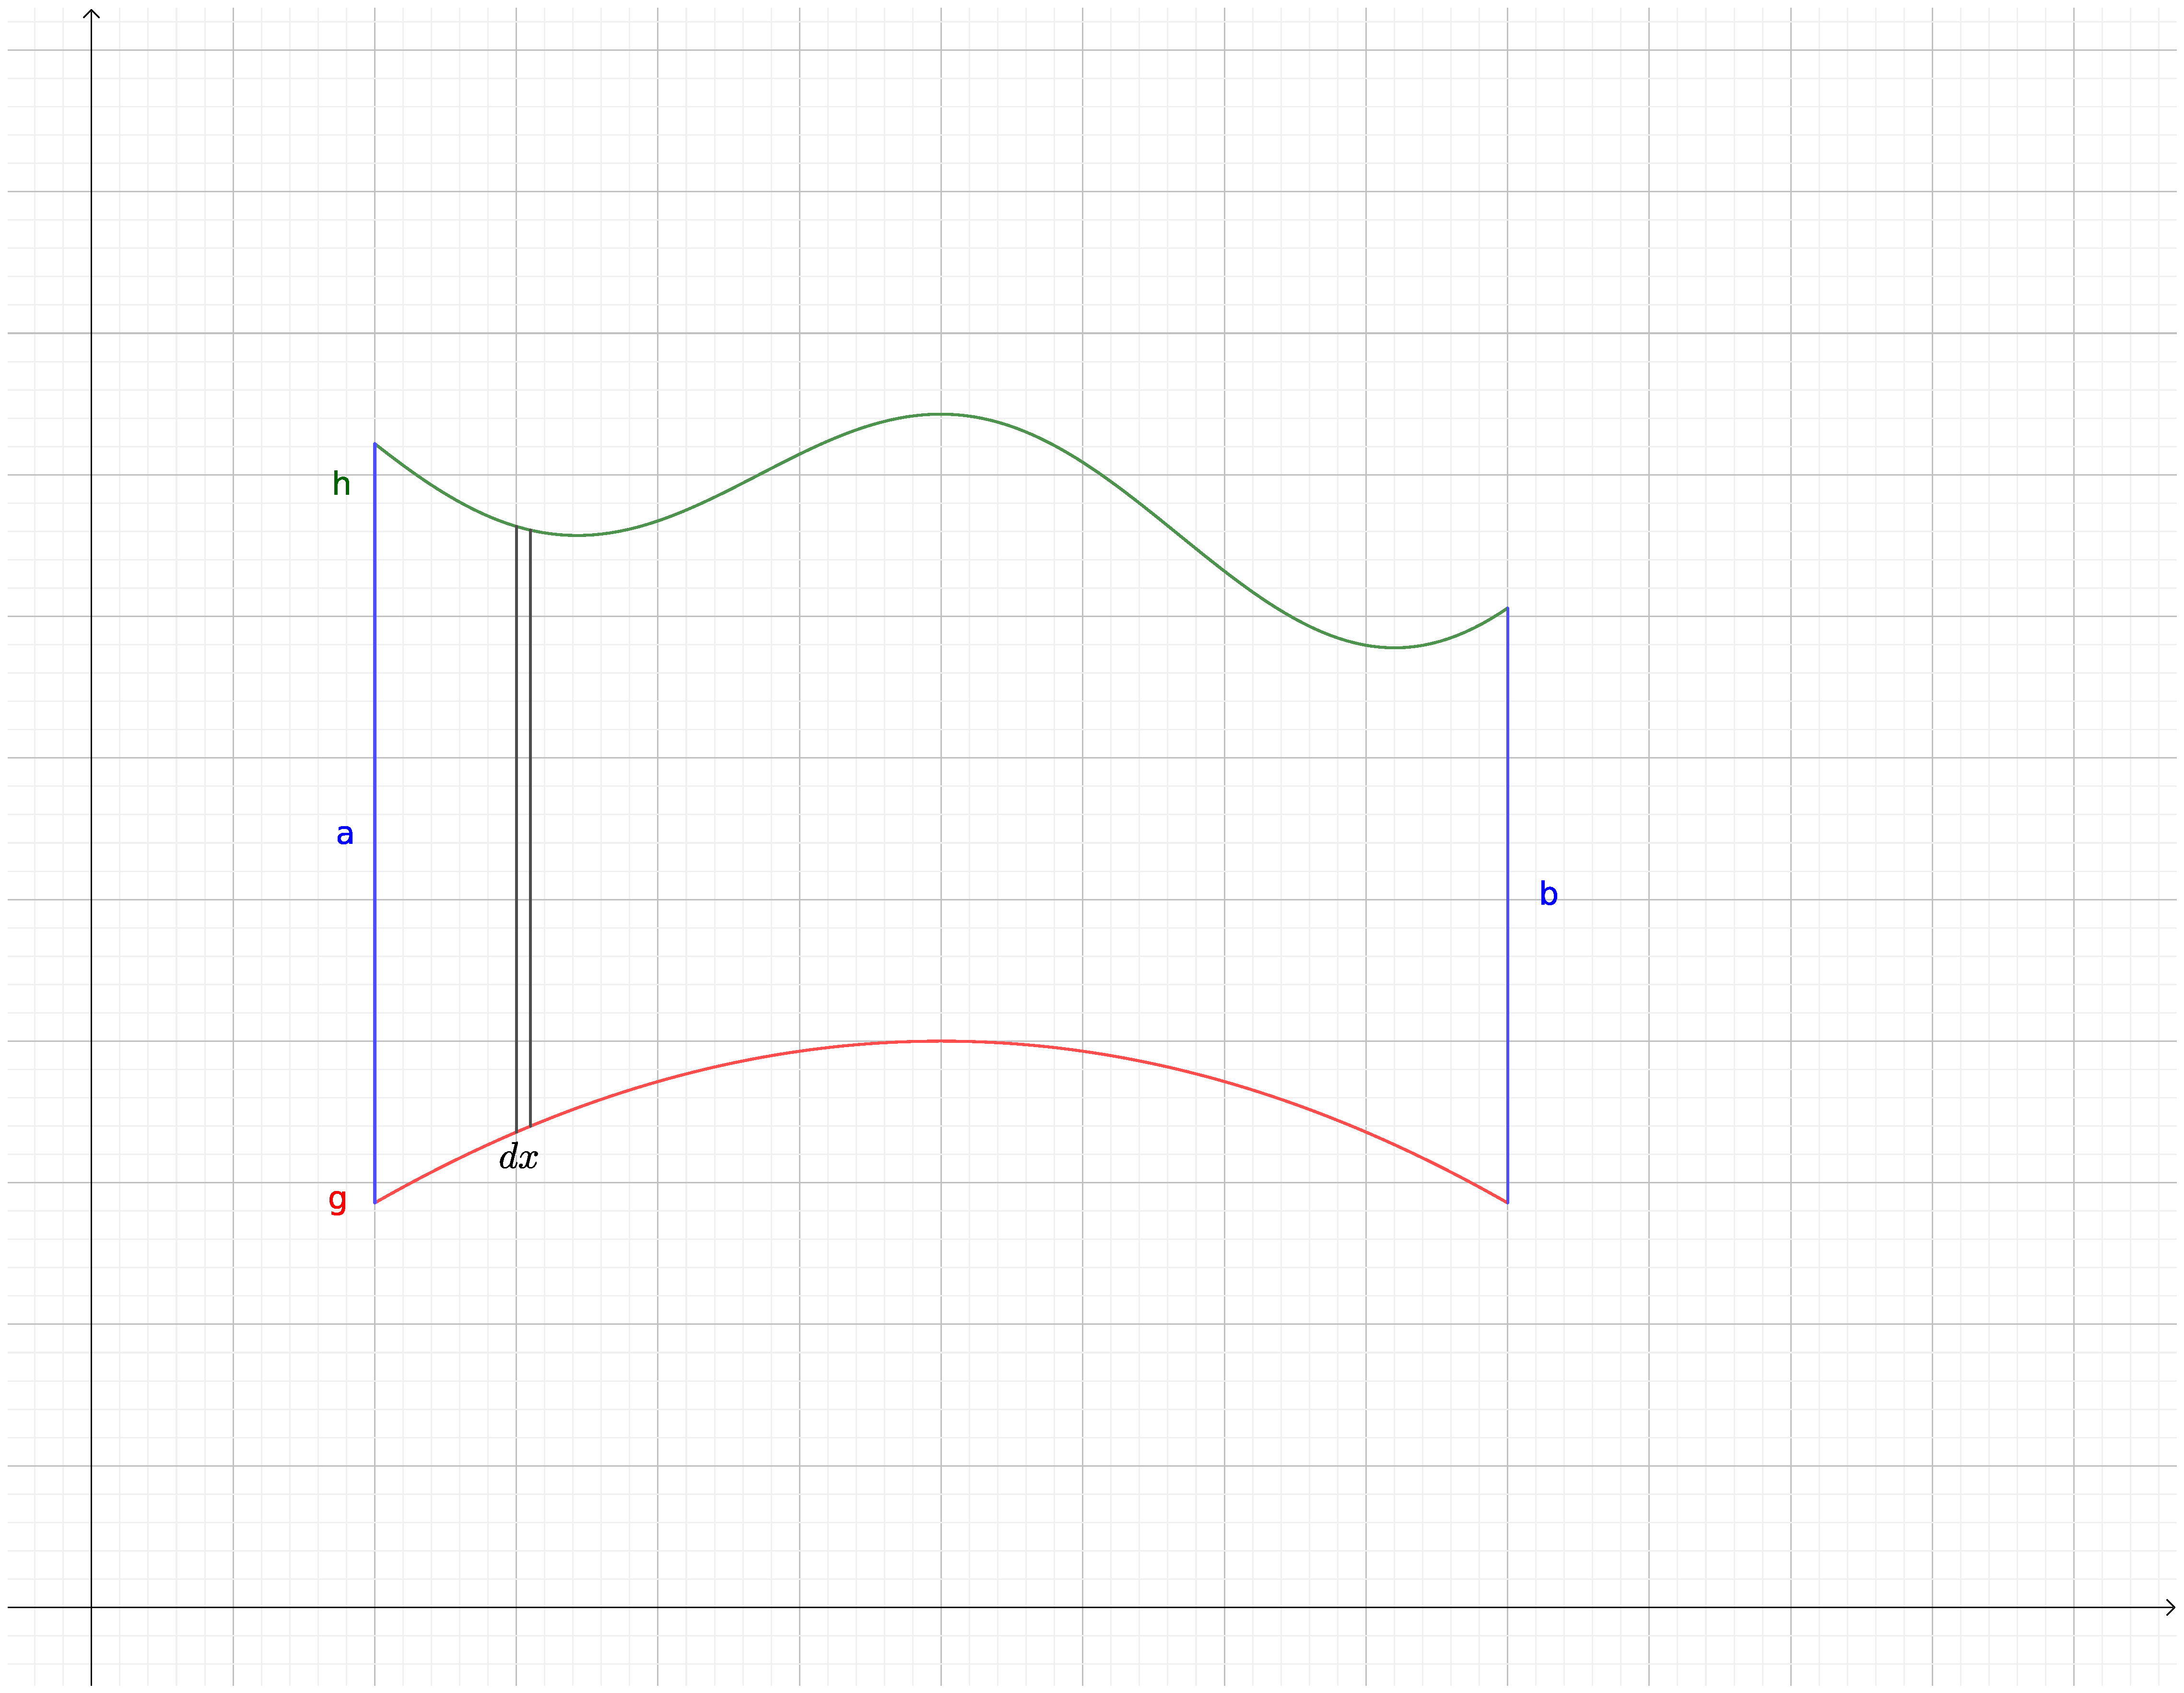
\includegraphics[width=0.45\textwidth]{y-simple.eps}
        \caption{An $x$ (left) and $y$-simple (right) region}
    \end{figure}\\\\
    Some regions in $\mathbb{R}^2$ are both $x$ and $y$-simple. However some regions in $\mathbb{R}^2$ are neither $x$ OR $Y$-simple. In such a case the region may be subdivided into $m$ non-overlapping regions each of which is $x$-simple, $y$-simple, or both. Let $D$ be a planar region. Assume $D$ is subdivided into $m$ non-overlapping regions where
    $$D=D_1\cup D_2\cup\cdots\cup D_m$$
    then if $f(x,y)$ is a function on $D$ then 
    $$\iint\limits_Df(x,y)\, dA=\iint\limits_{D_1}f(x,y)\, dA+\iint\limits_{D_2}f(x,y)\, dA+\cdots+\iint\limits_{D_m}f(x,y)\, dA$$  
    \subsection{Types of regions in $\mathbb{R}^3$}
    The description of a $z$-simple region in $\mathbb{R}^3$ is given. The description for $x$ and $y$-simple regions is similar.
    A region in three space is called $z$ simple if it is bounded from the bottom and top by the continuous surfaces $z=g(x,y)$ and $z=h(x,y)$ respectively. A $z$-simple region may be sliced vertically and hence is described by 
    $$E=\left\{\begin{array}{lr}
        g(x,y)\leq z\leq h(x,y)\\
        (x,y)\in B
    \end{array}\right.$$
    Where $B$ is a region in $\mathbb{R}^2$.
    \subsection{A definite partial integral}
    A definite integral of the form 
    $$\int\limits_{x=g(y)}^{x=h(x)}f(x,y)\, \partial x\ \ \mathrm{ or }\ \ \int\limits_{g(y)}^{h(y)}f(x,y)\, dx$$
    is a definite partial integral with respect to $x$. To compute the definite partial integral, integrate $f(x,y)$ with respect to $x$ but treating $y$ as constant. Definite partial integrals of three or more variables are defined similarly.
    \subsection{An Iterated Integral}
    An iterated integral consists of two or more definite partial integrals. For instance
    $$\int\limits_c^d\int\limits_a^b f(x,y)\, dx\, dy$$
    is an example of an iterated integral. To compute an iterated integral and evaluate outward.
    \subsection{Setting Up Limits for a Double Integral:}
    Given the double integral
    $$\iint\limits_D f(x,y)\, dA$$
    If region $D$ is a $y$-simple region. For a $y$-simple region, the region is sliced vertically, and hence to integrate over a $y$-simple region $dA$ is written,
    $$dA=dy\, dx$$
    It follows that the integral becomes
    $$\int\limits_a^b\int\limits_{g(x)}^{h(x)}f(x,y)\, dy\, dx$$

    If region $D$ is a $x$-simple region, the region is sliced horizontally, and hence to integrate over a $x$-simple region $dA$ is written,
    $$dA=dx\, dy$$
    It follows that the integral becomes
    $$\int\limits_c^d\int\limits_{p(x)}^{q(x)}f(x,y)\, dx\, dy$$
    \subsection{Setting up Limits for a Triple Integral}
    Consider the triple integral
    $$\iiint \limits_E f(x,y,z)\, dV$$
    Here assume that the region $E$ is $z$-simple. Setting up the limits for and $x$-simple or $y$-simple region is similar. Recall for $z$-simple regions they are sliced vertically and hence integrate with respect to $z$ first. That is
    $$dV=dz\, dA$$
    Once the inner most integral is computed, the triple integral is reduced to a double integral.
    \subsection{Geometric Interpretation of the Double Integral:}
    Consider the double integral
    $$\iint\limits_D f(x,y)\, dA$$
    for simplicity sake, we shall assume $f(x,y)\geq 0$ for $(x,y)\in D$. Let $S$ be the surface given by the equation $z=f(x,y)$, and let $V$ be the volume which lies vertically bellow $S$ and above the $xy$ plane on the region $D$. The slice $dA=dx\, dy$ is a small area on $D$. Therefore it is implied that
    $$V=\iint\limits_Df(x,y)\, dA$$
    In general where $f(x,y)$ is not necessarily greater than or equal to zero. In general the triple integral, 
    $$\iiint\limits_Ef(x,y,z)\, dV$$
    is the signed hyper volume in four dimensional space. If $f(x,y)=1$ on $D$ then the integral reduces to
    $$A=\iint\limits_D dA$$
    and gives the area of $D$. If $f(x,y,z)=1$ in the region $E$ then the integral reduces to
    $$V=\iiint\limits_EdV$$
    and gives the volume of the region $E$. This implies that a volume can be computed by either a double or triple integral.
    \subsection{Polar, Cylindrical and Spherical Coordinate Systems:}
    \subsubsection{Polar Coordinates System:}
    \begin{wrapfigure}{r}{0.5\textwidth}
        \vspace{-20pt}
        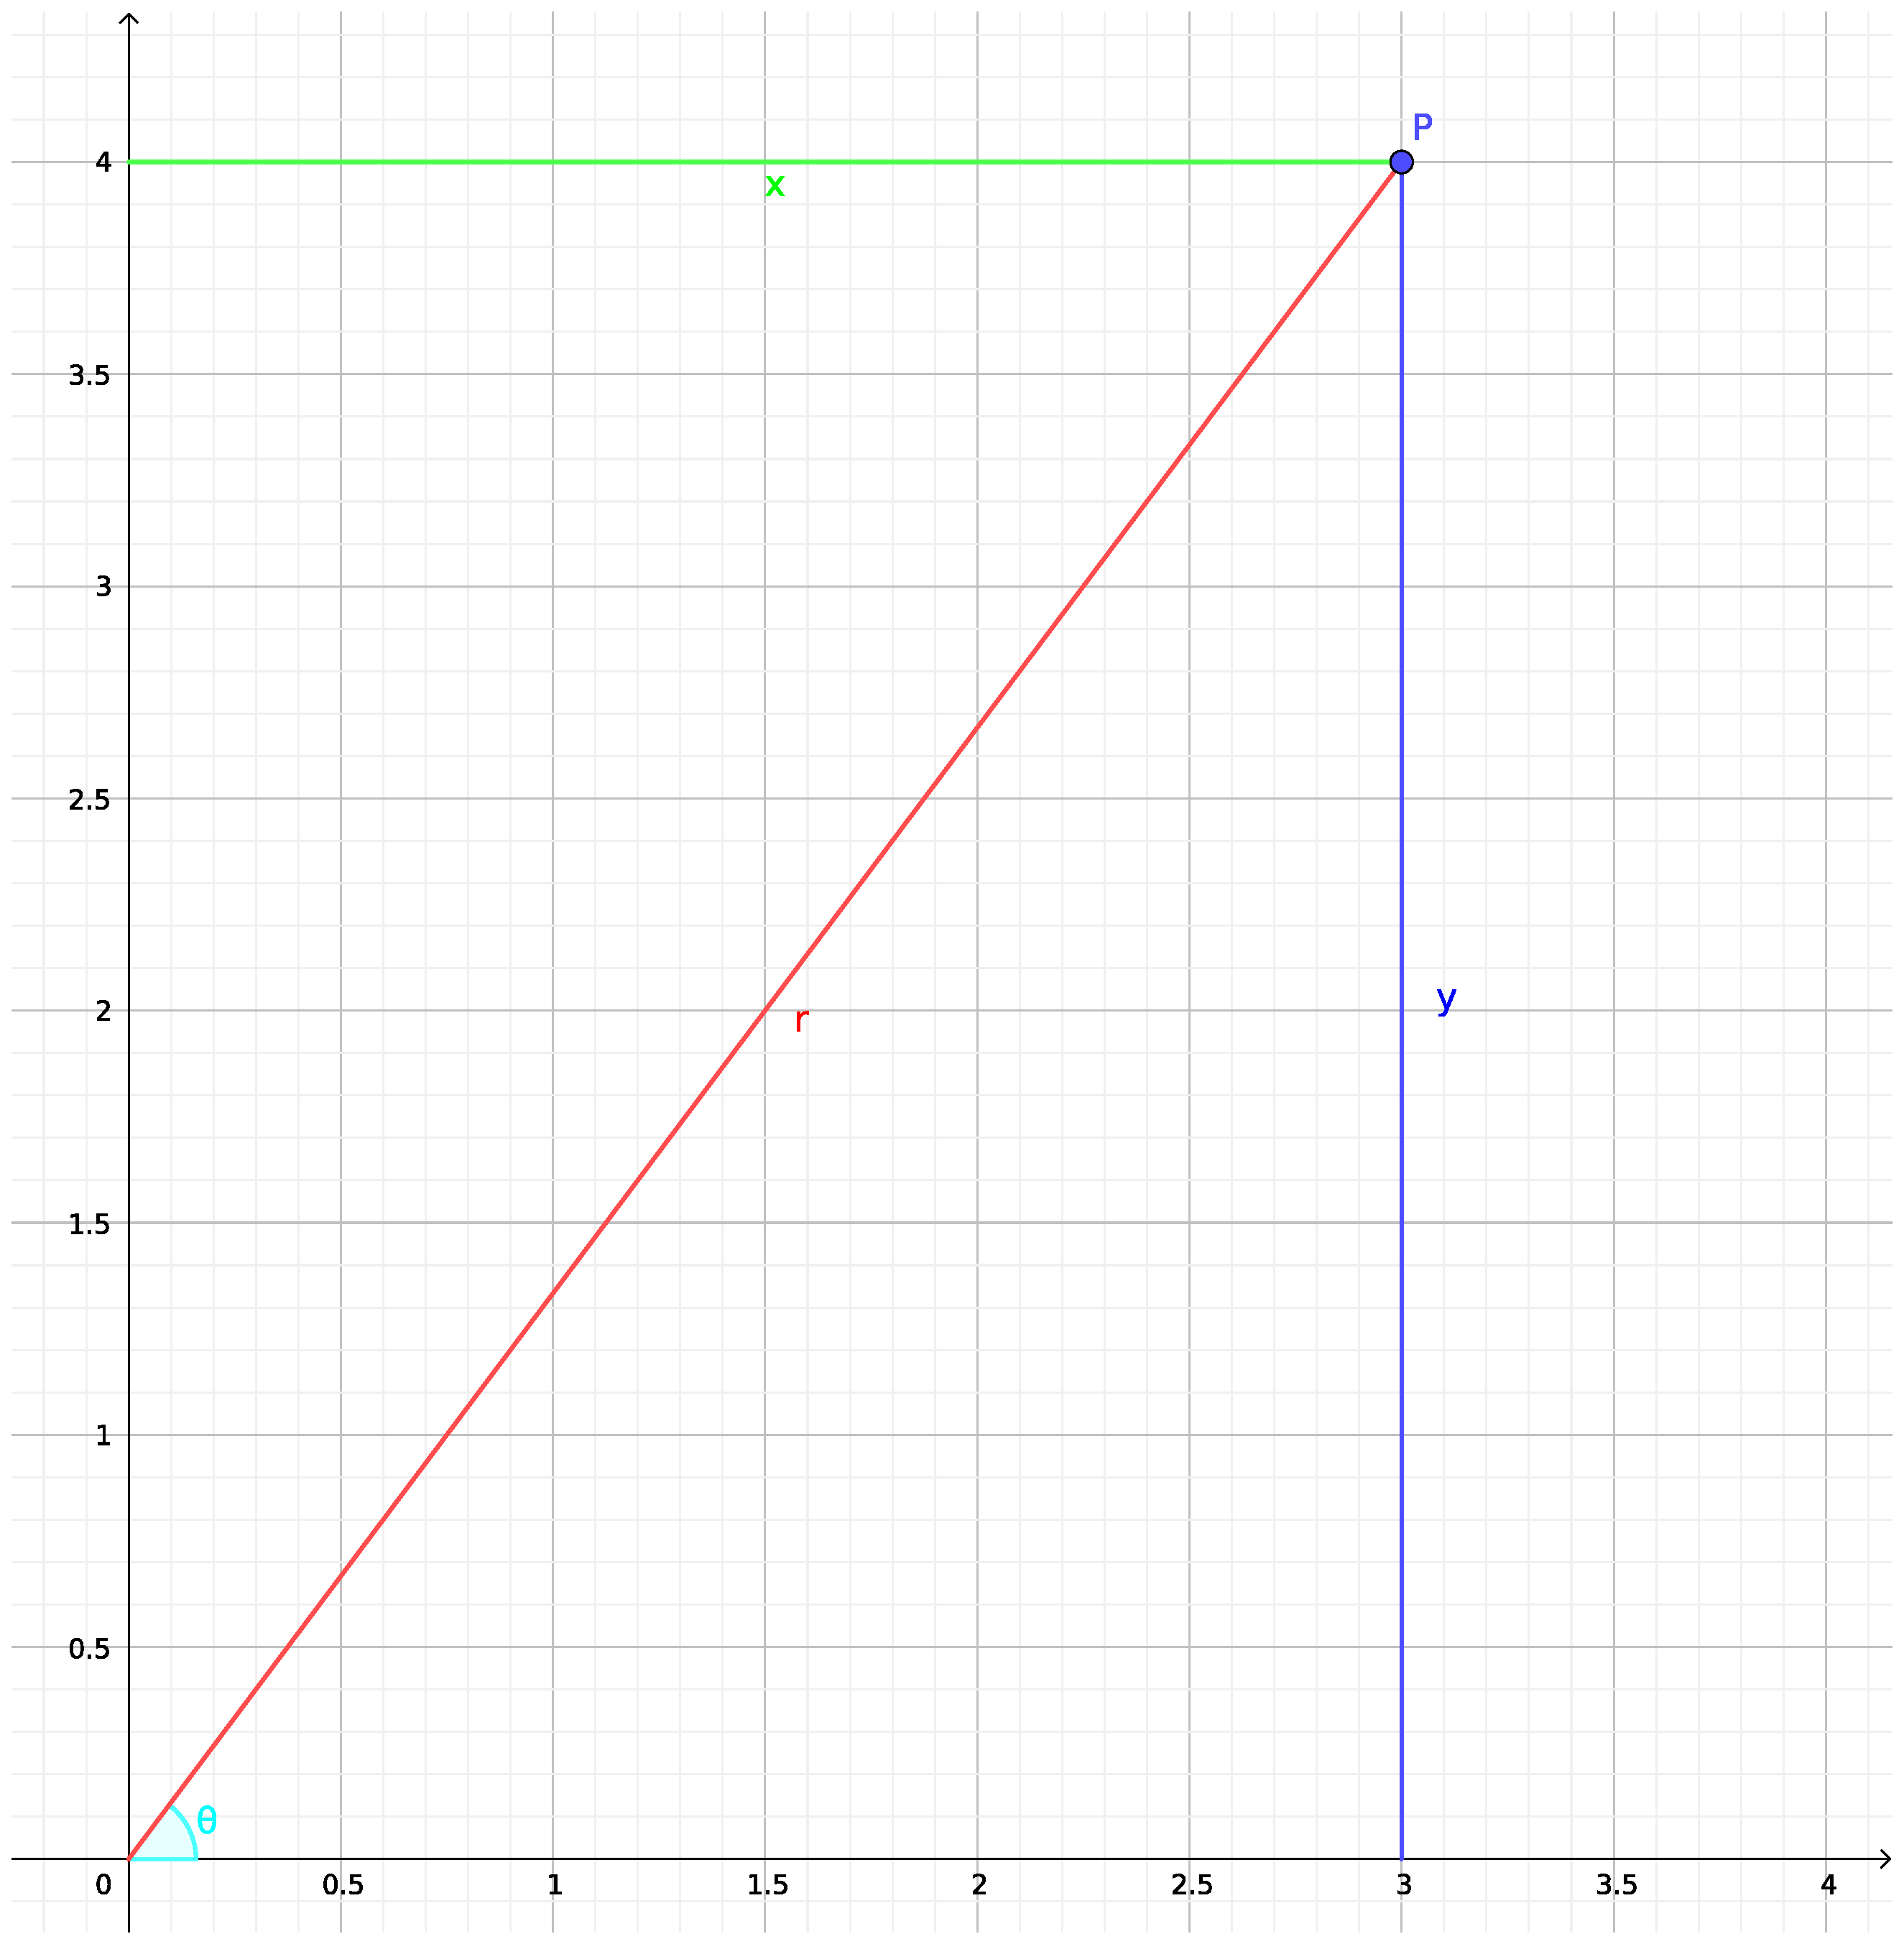
\includegraphics[width=0.45\textwidth]{polarCord.eps}
        \vspace{-20pt}
    \end{wrapfigure}
    Let $P(x,y )$ be a point in the $xy$-plane. The polar coordinates of $P$ are $r$, and $\theta$ where $r$ is the distance between the origin and the point $P$ and $r\in[0, \infty)$ and $\theta$ is the angle between $\vec{OP}$ and the positive $x$-axis and $\theta\in[0, 2\pi]$. The cartesian and polar coordinates are usually displayed on the same figure as shown and have the following relationships,
    \begin{align*}
        x=r\cos\theta\\
        y=r\sin\theta\\
        r^2=x^2+y^2\\
        \frac{y}{x}=\tan\theta\\
        dA=r\, dr\, d\theta
    \end{align*} 
    \subsubsection{Cylindrical Coordinate System:}
    The cylindrical coordinate system is a three dimensional version of polar coordinates.\\ The point $P(x,y,z)$ is $(r, \theta, z)$ in cylindrical coordinates.
    \subsubsection{Spherical Coordinate System} 
    The spherical coordinate system is closely related to the geographical longitudes and latitudes. Let $P(x,y,z)$ be a point of the surface of a sphere. The spherical coordinates of $P$ are $\rho$, $\phi$, and $\theta$ where where $\rho$ is the distance from the origin to $P$ with $\rho\in[0,\infty)$, $\phi$ is the angle made between $\vec {OP}$ and the positive $z$-axis with $\phi\in[0, \pi]$ and $\theta$ is the angle made between $\vec{OQ}$ and th positive $x$-axis with $\theta\in[0,2\pi]$.
    \begin{align}
        x=r\cos\theta\label{rx}\\
        y=r\sin\theta\label{ry}\\
        r^2=x^2+y^2\label{r2}\\
        r=\rho\sin\phi\label{rrho}\\
        z=\rho\cos\phi\label{zrho}\\
        \rho^2=z^2+r^2\label{rho2}
    \end{align}
    Substitute \eqref{rrho} into \eqref{rx}, \eqref{ry}, \eqref{r2}, and \eqref{rho2}, to obtain,
    \begin{align*}
        x=\rho\,\sin\phi\,\cos\theta\\
        x=\rho\,\sin\phi\,\sin\theta\\
        z=\rho\cos\phi\\
        \rho^2=x^2+y^2+z^2\\
        x^2+y^2=\rho^2\sin^2\phi\\
        dV=\rho^2\sin\phi\,d\rho\, d\phi\, d\theta
    \end{align*}
    When the equations describing a region $D$ contain $x^2+y^2$, substitute $x^2+y^2=r^2$ and use polar or cylindrical coordinates. When the equation describing a region $E$ contains $x^2+y^2+z^2$, substitute $x^2+y^2+z^2=\rho^2$, and use spherical coordinates.
    \subsubsection{A special Curve in Polar Coordinates:}
    The equation of a circle centered at $(0,0)$ and with radius $a$ is given by 
    $$x^2+y^2=a^2$$
    in polar coordinates $r^2=x^2+y^2$ so therefore $r^2=a^2$, or
    $$r=a$$
    \subsubsection{A special Surface in cylindrical Coordinates}
    Recall that a cylinder can be given by any curve in $\mathbb{R}^2$ projected into $\mathbb{R}^3$. Therefore the right circular cylinder is given by the equation of a circle. From above it can be seen that a circular cylinder in cylindrical coordinates, centered at $(0,0)$, and with radius $a$ can be given by,
    $$r=a$$
    \subsubsection{Three Special Surfaces in Spherical Coordinates:}
    \begin{enumerate}
        \item The equation of a sphere of radius $a$ centered at $(0,0,0)$ is given by 
        $$x^2+y^2+z^2=a^2$$
        in spherical coordinates $x^2+y^2+z^2=\rho^2$
        $$\therefore \rho=a$$
        \item The equation of a sphere of radius $a$ with center $(0,0,a)$ is given by 
        \begin{align*}
            x^2+y^2+(z-a)^2&=a^2\\
            x^2+y^2+z^2&=2az
        \end{align*}
        In spherical coordinates $z=\rho\cos\phi$ and $x^2+y^2+z^2=\rho^2$, 
        \begin{align*}
            \therefore\rho^2&=2a\rho\cos\phi\\
            \rho=2a\cos\phi
        \end{align*}
        \item The equation of a cone is given by
        $$z=\alpha \sqrt{x^2+y^2}$$
        in spherical coordinates $z=\rho\cos\phi$ and $x^2+y^2=\rho^2\sin^2\phi$, so
        \begin{align*}
            \rho\cos\phi&=\alpha\sqrt{\rho^2\sin^2\phi}\\
            \therefore \phi&=\tan^{-1}\left(\frac{1}{\alpha}\right)
        \end{align*}
    \end{enumerate}
    \subsubsection{Setting Up Limits of Integration in Polar Coordinates:}
    Given the double integral
    $$\iint\limits_Df(x,y)\,dA$$
    To compute using polar coordinates, apply the following three steps,
    \begin{enumerate}
        \item In the expression of $f(x,y)$, replace $x$ by $r\cos\theta$, $y$ by $r\sin\theta$, and $x^2+y^2$ by $r^2$.
        \item Replace $dA$ by $r\, dr\, d\theta$
        \item Express $D$ in polar coordinates.
    \end{enumerate}
    \subsection{Application of Double and Triple Integrals in Calculating Mass, Moments, Centers of Mass, and Centroids}
    Let $D$ be the planar region occupied by a thin plate or lamina. Assume that the plate is not uniform and that the area density is given by the function
    $$\delta(x,y)$$
    The mass is given by definition as the sum of the elements of mass
    $$dm=\delta(x,y)\, dA$$
    The mass is given by 
    $$m=\iint\limits_D\delta(x,y)\, dA$$
    The moment about the $y$ axis may be denoted $M_{x=0}$. By definition the element of moment about the $y$-axis is
    $$dM_{x=0}=x\, dm$$
    The total moment is then given by,
    $$M_{x=0}=\iint\limits_D x\, dm$$
    likewise the moment about the $x$-axis is 
    $$M_{y=0}\iint\limits_D y\, dm$$
    The center of mass $(\bar x, \bar y)$ is an imaginary point where the entire mass is assumed to be concentrated. By definition
    \begin{align*}
        M_{x=0}=\bar x m&\Rightarrow\bar x=\frac{M_{x=0}}{m}
        M_{y=0}=\bar y m&\Rightarrow\bar y=\frac{M_{y=0}}{m}
    \end{align*} 
    If the lamina is uniform then its density is constant\footnotemark[2]
    $$\delta(x,y)=C$$
    In such a case, the center is mass is referred to as a centroid. Likewise let $E$ be the region in three space occupied by a solid. Assume the solid is not uniform and that the density function is
    $$\delta(x,y,z)$$
    The mass is given by
    $$m=\iiint\limits_E dm$$
    The moment about the $yz$-plane is
    $$M_{x=0}=\iiint\limits_E x\, dm$$
    The moment about the $xz$-plane is
    $$M_{y=0}=\iiint\limits_E y\, dm$$
    The moment about the $xy$-plane is
    $$M_{z=0}=\iiint\limits_E z\, dm$$
    The center of mass $(\bar x, \bar y, \bar z)$ is given by
    \begin{align*}
        \bar x=\frac{M_{x=0}}{m}&&\bar y=\frac{M_{y=0}}{m}&&\bar z=\frac{M_{z=0}}{m}
    \end{align*}
    if $\delta(x,y,z)$ is constant\footnotemark[2] then the center of mass is the centroid. In all equations above $dm=\delta(x,y,z)\, dV$. 
    \footnotetext[2]{{It is generally assumed in this case that the density is equal to 1}}
\end{document}